% smrdoc.tex V2.10, 13 July 2012

\documentclass[a4paper]{article}
\usepackage{geometry}
\geometry{left=2.5cm,right=2.5cm,top=2.5cm,bottom=2.5cm}
\usepackage{moreverb}
\usepackage{epsfig}
\usepackage[colorlinks,bookmarksopen,bookmarksnumbered,citecolor=red,urlcolor=red]{hyperref}
\usepackage{listings}
\usepackage{amsmath}
\usepackage{amsfonts}
\usepackage{amssymb}
% For table
\usepackage{booktabs}
\usepackage{array}

% Include extern styles
\usepackage{extern-styles/nasm/lang}
\usepackage{extern-styles/nasm/style}

\usepackage{color}
\usepackage[lined, linesnumbered, boxed, ruled, commentsnumbered]{algorithm2e}


\begin{document}
\title{Making Fuzz Testing Smarter Again}
\author{Beary, Hu Dou}
\maketitle

\begin{abstract}
% Vulnerbility is very critical. Fuzz testing is a very popular in finding bugs. While this method is quit dumb when compared with symbolic execution.
% In order to improve the ability of fuzz testing itself, we proposed seed prioritization method to select most promising seed to be mutated first. Then fuzz testing cannot test deeper code blocks which we use hybrid testing method to assit it. 
% We implemented the prototype and evaluated it on some real-world binaies to demonstrate its effectiveness and efficiency. The experiments results show our prototype can be smarter than some other vulnerability discovery tools.

% FIXME:
Fuzz testing is a popular method to discover the bugs and vulnerabilities in software. However, traditional fuzz testing still faces the low coverage and fewer efficiency problems when testing real-world binary executables. Treating the program as a black-box makes it harder for fuzz testing to steer the program into deeper state space. In this paper, we improved the ability of fuzz testing itself by prioritizing the seed queue in coverage based evolutionary testing. Meanwhile, we took the advantage of hybrid testing method to improve the coverage with the assistance from symbolic execution. We have proposed two main optimizations to improve the ability of hybrid testing method. We also designed and implemented a prototype tool -- Beary on top of fuzz testing and symbolic execution, and the experiments results on real-world binary software have demonstrated that our method can make the fuzz testing more smarter when compared with other vulnerability discovery tools.
% Need to be refactored

\end{abstract}
\textbf{Keywords.} Fuzz Testing; Symbolic Execution; Vulnerability; Hybrid Testing Method

\section{Introduction}
Software errors and vulnerabilities have brought critical threaten to not only individuals but also for the whole cyber security. Despite the software quality of software engineering has ever-increasing, some software vulnerabilities still can be found every year by researchers both in academia and industrial communities. 

Even though some software errors and vulnerabilities can be discovered manually, manual analysis is still not a scalable method for large-scale software. During the past several years, many automatic methods have been proposed to improve the dependability of software before and after the software have been released, like source code auditing, fuzz testing, symbolic execution. However, all of these methods still need to solve some obstacles before they can be well applied to large-scale real-world software.

Source code auditing is a powerful methodology for locating security vulnerabilities in source code. However, the need to access source code prevents it from being deployed onto binary software testing to detect vulnerabilities in the released binary executables. 
  
 needs to access source code which prevent it from being deployed onto binary software testing. And even though it can obtain more information from the source code than binary, it still cannot make sure there are no vulnerabilities in the released binary executables. Fuzz testing is used to automatically discover vulnerabilities in binary executables and it is the most popular technique in the industrial community and according to the [XXX], most of the vulnerabilities in CVE and NVD databases are discovered by fuzz testing. However, a large portion of released fuzzing tools treats the target software as a black box which means they simply feed the target binaries with randomly generated test cases. And obviously, only a very small portion of the randomly generated test cases can trigger new behaviors of the target binary by touching new paths or basic blocks. While most of the test cases are proved as redundant and there has no doubt that black box fuzz testing faces a serious efficiency problem.

Symbolic execution is an analysis method to automatically generate an input that can drive some specific code region to be executed. Symbolic execution interprets the target program by assigning symbolic data rather than concrete data to the program inputs and then uses SAT solvers to generate test cases that satisfy with both branches when encountering a branch. However, the "path explosion" problem impedes symbolic execution from applying to real-world software. During the recent years, some improvements have been made to help symbolic execution to be adaptable to real-world testing, like, selective symbolic execution and so on. Selective symbolic execution bounds the number of execution states though "elastic" expanding the program execution path. Selective symbolic execution has eased the ?path explosion? problem to some extent and made it possible for applying symbolic execution to real-world software. And based on such improvements, some automatic symbolic execution tools have been developed, such as EXE, KLEE, SAGE, Mayhem, S2E and Angr. 

We realized that even the state of the art effective technique base on program analysis is less efficient than black box fuzzing if the time spent generating a test case take relatively too long. Symbolic execution has to spend the most time on program analysis and constraint solving, while black box fuzzing only concentrate on random mutations. In this paper, we aim to improve the performance of fuzz testing by adding two main features for fuzz testing. We proposed a similarity based seed searcher for fuzz testing to speed up the path discovery, and we also leveraged symbolic execution to improve the coverage of fuzz testing by selectively solving the branches which are guarded by complex conditions. And we also present our prototype which is built on top of our method. Furthermore, some additional evaluations are performed to demonstrate the ability of our methods \cite{patashnik-bibtexing}.
 
In summary, this paper makes the following contributions.
\begin{itemize}
\item We proposed a novel method to prioritize the seed files for fuzz testing to speed up the path discovery.

\item We propose a novel method based on lazy forking to handle the \emph{symbolic pointers} when using symbolic execution to assist fuzz testing.

\item We designed and built the prototype for our method to demonstrate our approaches.

\item We evaluate our method and prototype on several benchmarks to demonstrate the effectiveness and efficiency from several different viewpoints.
\end{itemize}

\section{High Level Overview}
\begin{figure}
\centering
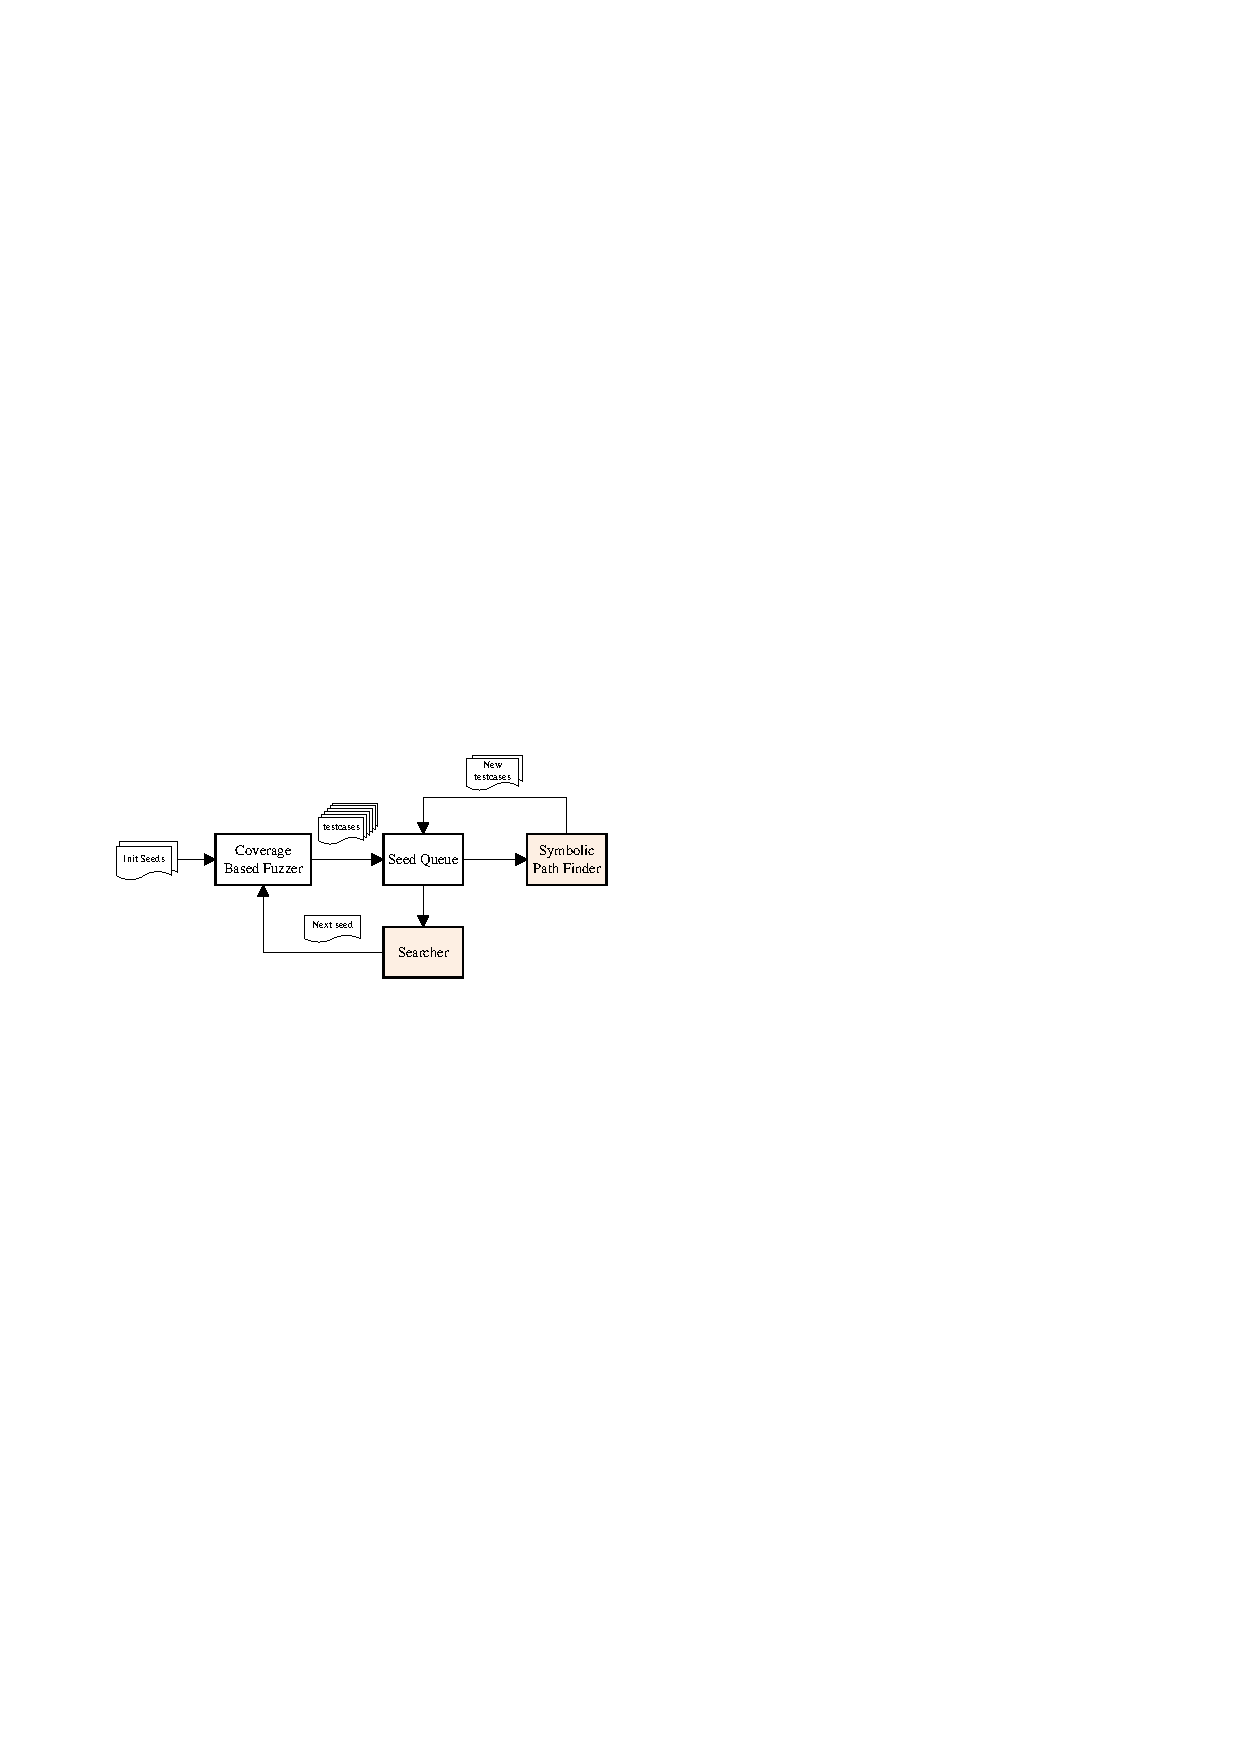
\includegraphics[width=0.7\textwidth]{figures/framework.pdf} 
\caption{High Level Framework.}\label{Framework}
\end{figure}

% TODO: Making this part more clear?

Figure~\ref{Framework} shows the basic framework of our system. From a high-level scope, our method is built on top of a coverage based fuzzer. 
The fuzzer accepts some initial seed files as inputs and produces a seed queue by collecting the mutated test cases that trigger new behaviors of the target program. 
Our main contributions, which consists of two components, namely \emph{Seacher} and \emph{Concolic Path Finder}, focus on improving the quality of the seed queue. 
Traditional coverage based fuzz testing will pick up seed files from the seed queue one by one as the new seed file to mutate. However, this strategy faces the efficiency problem when testing modern software that have a huge state space. This means the test case will be very huge and mutating each test case in the queue will consumes lots of time. The \emph{Searcher} is designed to select the most promising seed file from the seed queue based on the distance measurement. The most promising seed file is the seed file that has the longest average \textit{distance} from all other seed files in the queue. By doing this, the fuzzer will touch more virgin code areas to improve the coverage as soon as possible in a time budget. 
The \emph{Concolic Path Finder} is leveraged to help the fuzzer to dive into deeper code areas that guarded by complex path constraints. This is achieved by solving the uncovered branches along with the seed files in the queue. All the test cases generated by \emph{Concolic Path Finder} will be added to the seed queue to find more paths.


\section{Seed Prioritization for Fuzz Testing}
As mentioned before, the size of the seed queue of coverage based evolutionary fuzz testing will quickly reach a large number (especially with the assistance of symbolic execution) when testing large-scale modern software. The seed queue should be rearranged to make sure we can find more paths when given a fixed time budget.

%TODO: Add the legend of the coverage area of initial seed file in the figure

%TODO: Add maximize memory coverage
We realized that different seed files in the queue have different power of finding new paths. For example in Figure~\ref{motivate-example}, suppose the state space of a program is modeled as a two-dimensional space, and each input that triggers new behavior will be mapped to a specific dot in the space. The fuzz test starts from an initial seed which is marked as red in this figure. The mutation results of this initial seed cover the black points as well as seed A and seed B. Then, in evolutionary fuzz testing, a test case will be picked up as the seed file for next round of mutation. 
Consider the choice between seed A and B in this figure, the \emph{distance}(eg. Euclidean Distance) from the initial seed file to A is much shorter than B, which, in other words, means that A is more \textbf{\textit{similar}} to the initial seed file than B. So choosing A as the next seed file to mutate will only trigger two new paths as most of the mutated test cases are (the blue area) overlapped by what the initial seed has mutated (the gray area). However, because seed B has a longer distance from the initial seed than seed A, the coverage area of B (the brown area) will have less overlap by that of initial seed file than A. So choosing seed B will trigger more new behaviors than selecting seed A.


Based on this insight, we proposed a test case prioritization method based on \emph{distance} between test cases. Our method investigated three distance measures, i.e. \textit{Euclidean Distance}, \textit{Cosine Similarity} and \textit{Jaccard Index}, as the classification metrics for test case prioritization. Each test case in the seed queue will be assigned with a \emph{weight} value after being mapped as a vector from input space to state space. The \emph{weight} value is utilized as the criteria to determine which seed file should be scheduled as the next seed through a global optimum solution.

In the following sections, we firstly introduce these three distance metrics and then explain how a test case is mapped to a numerical vector as well as the seed prioritization method.

\begin{figure}
\centering
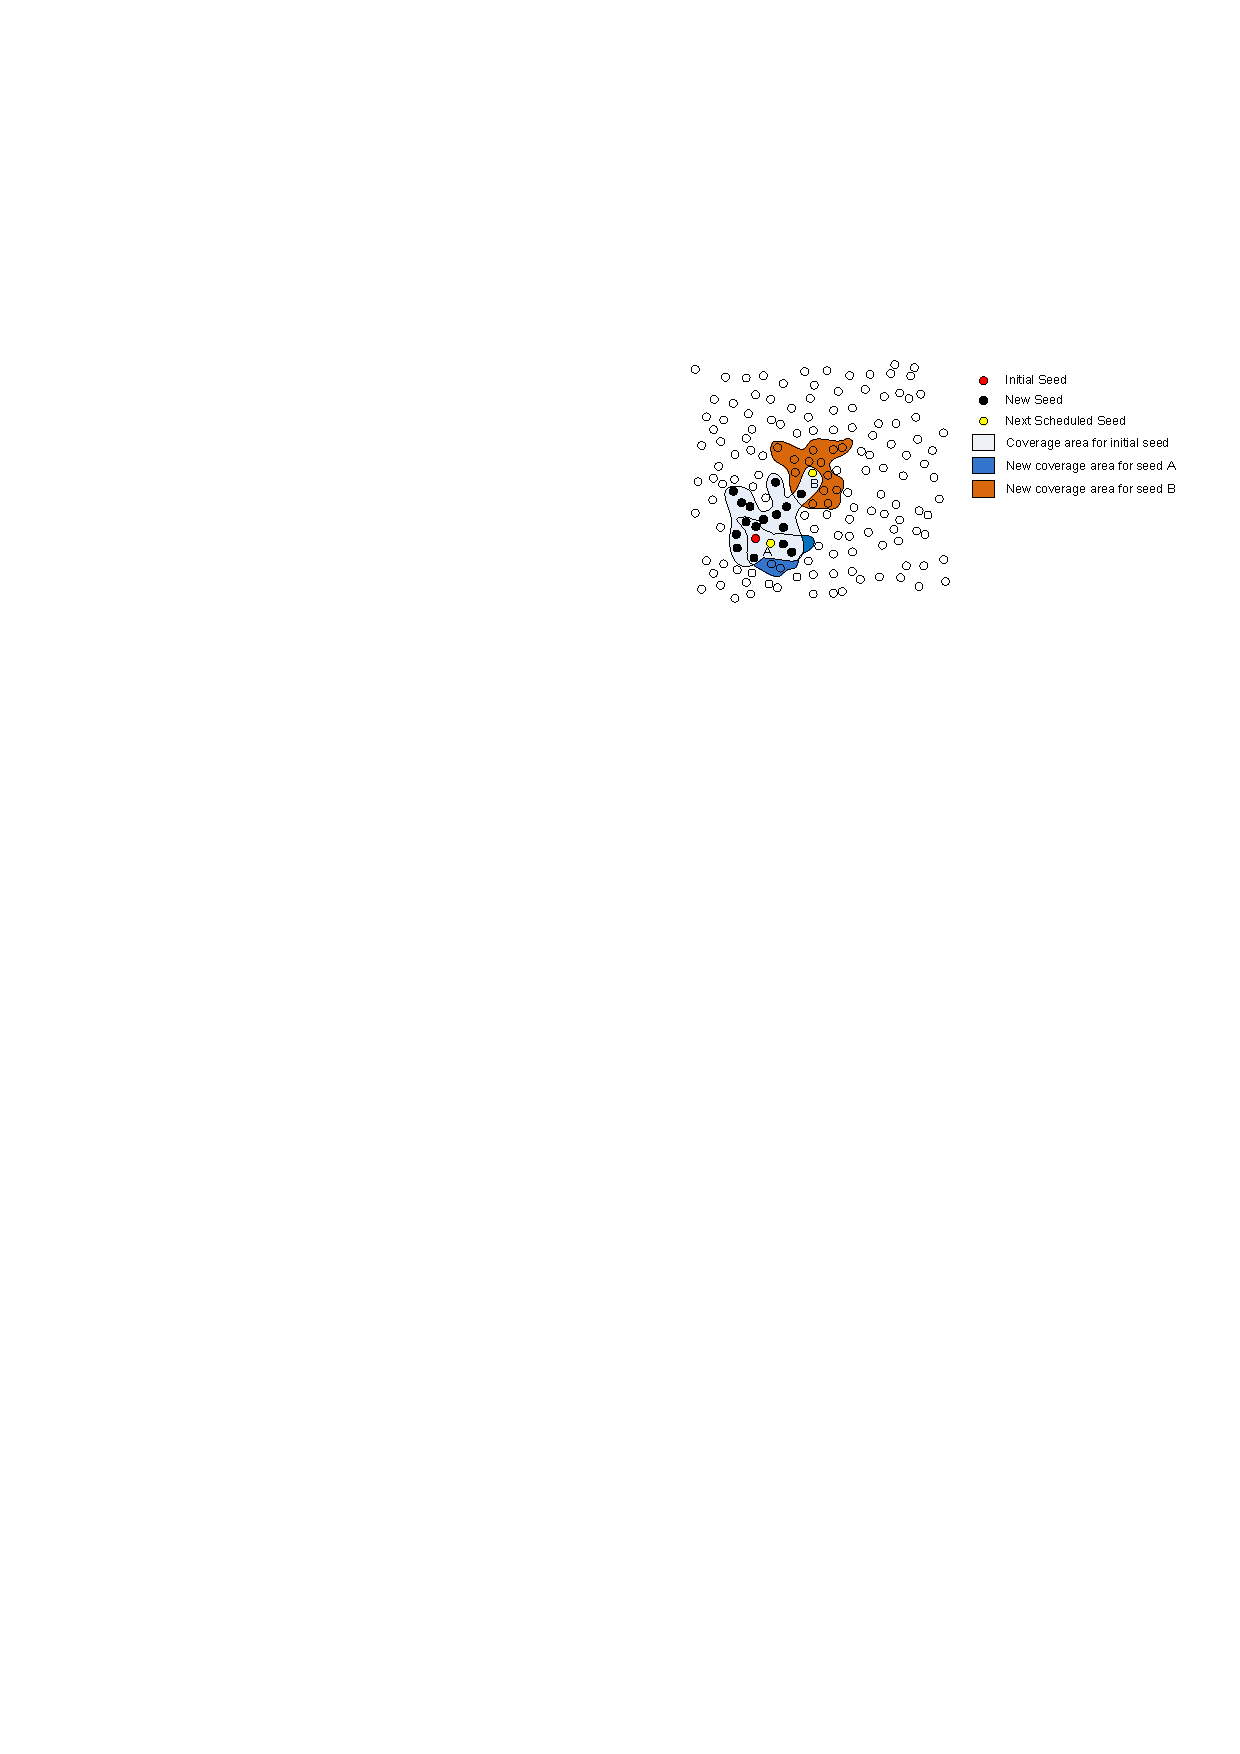
\includegraphics[width=0.7\textwidth]{figures/motivate-example.pdf} 
\caption{A motivating example.}\label{motivate-example}
\end{figure}

\subsection{Distance Metrics}
For two vectors $\mathit{X} = (x_1, x_2, \cdots, x_N)$ and $\mathit{Y} = (y_1, y_2, \cdots, y_N)$, the corresponding similarity metrics for \textit{Euclidean Distance}, \textit{Cosine Similarity} and \textit{Jaccard Index} are listed as follows.

\begin{enumerate}
\item Euclidean Distance (EU)

The Euclidean Distance between two vectors is defined as follows:
\begin{center}
$EU(\mathit{X}, \mathit{Y}) = \displaystyle \sqrt{\sum_{i=1}^{N} (x_i-y_i)^2}$
\end{center}


\item Cosine Similarity (CS)

The consine similarity between $\mathit{X}$ and $\mathit{Y}$ is defined as follows:

\begin{center}
$CS(\mathit{X}, \mathit{Y}) = \displaystyle \sqrt{\frac{\mathit{X}^T \cdot \mathit{Y}} {\| \mathit{X} \|\| \mathit{Y} \|}}$
\end{center}
where $\mathit{X}^T$ is a transposition of vector $\mathit{X}$ and $\| \mathit{X}\|$ is the Euclidean Distance of
vector $\mathit{X}$. Similarly, $\|\mathit{Y}\|$ is the Euclidean norm of vector $\mathit{Y}$. In essence, \textit{CS} is the cosine of the angle between $\mathit{X}$ and $\mathit{Y}$ in the N-dimensional space. For cosine similarly, the corresponding distance is defined as:

\begin{center}
$D(\mathit{X},\mathit{Y}) = 1 - CS(\mathit{X},\mathit{Y})$
\end{center}

\item Jaccard Index (JI)

The Jaccard Index between $\mathit{X}$ and $\mathit{Y}$ is defined as follows:

\begin{center}
$JI(\mathit{X}, \mathit{Y}) = \displaystyle \frac{\mathit{X} \cdot \mathit{Y}}{\mathit{X} \cdot \mathit{Y}+\omega(\|\mathit{X}\|^2+\|\mathit{Y}\|^2-2(\mathit{X} \cdot \mathit{Y}))}$
\end{center}

where $\mathit{X} \cdot \mathit{Y}$ is the inner product of $\mathit{X}$ and $\mathit{Y}$. 
When $\omega$ is equal to 1, the above formula is called Jaccard index and its corresponding distance is defined as follows:

\begin{center}
$D(\mathit{X},\mathit{Y}) = 1 - JI(\mathit{X},\mathit{Y})$
\end{center}

\end{enumerate}

\subsection{Seed Selection Method}
In order to measure the distances between test cases, all the test cases should be mapped to vector space. 
The mapping can be performed both from input space and state space. However, mapping from input space cannot reflect the real relationship between test cases when considering the behavior of the target program. For example, as shown in Figure~\ref{distance-illusion}, multiple different inputs can steer the program to execute the same path. Specifically, considering the three test cases namely \texttt{A.jpeg}, \texttt{B.jpeg} and \texttt{C.jpeg} in this figure, suppose the corresponding contents are shown as follows:
\\
\\
\indent\texttt{A.jpeg}: \texttt{$\backslash$xFF$\backslash$xD8$\backslash$xAA$\backslash$xBB$\backslash$xCC$\backslash$xDD}

\texttt{B.jpeg}: \texttt{$\backslash$xFF$\backslash$xD8$\backslash$xDD$\backslash$xCC$\backslash$xBB$\backslash$xAA}

\texttt{C.jpeg}: \texttt{$\backslash$xFE$\backslash$xD8$\backslash$xAA$\backslash$xBB$\backslash$xCC$\backslash$xDD}
\\

\indent Obviously, if we calculate the \textit{Euclidean Distance} between these three files based from input space, $ED_{AB}$ will be greater than $ED_{AC}$ because there are more different bytes between \texttt{A.jpeg} and \texttt{B.jpeg} than that of \texttt{A.jpeg} and \texttt{C.jpeg}. This means \texttt{A.jpeg} and \texttt{C.jpeg} are more similar (as shown in Figure~\ref{distance-illusion}) from the viewpoint in the input space. 
However, for most of the JPEG process programs, \texttt{A.jpeg} and \texttt{B.jpeg} will execute the same path. However, \texttt{C.jpeg} will execute another path because \texttt{C.jpeg} is an illegal JPEG file (bad magic number). So from the viewpoint of program, \texttt{A.jpeg} and \texttt{B.jpeg} are more similar than \texttt{A.jpeg} and \texttt{C.jpeg} even though \texttt{A.jpeg} and \texttt{C.jpeg} have only one bit difference. 
Since our objective is to maximize the coverage in the state space, so we choose to map all the test cases from the state space to numeric vectors to calculate the distance.

In \cite{wang2015similarity} all test cases are represented as a branch coverage vector $\mathit{V}=(v_1, v_2, \cdots, v_N)$, where $v_i$ is 0 means the branch is covered, otherwise 1. 
However, different test cases can affect different branches, so the mapped vectors may have different lengths which cannot be used directly for distance calculation. Meanwhile, it will be very difficult to construct such vectors because it is hard to obtain all the branches and list them orderly in each vector to avoid obfuscation between vectors. 
In AFL \cite{online:afl}, the execution path information of each test case is recorded into a \emph{Bitmap}. This \emph{Bitmap} is then used to determine whether a test case triggers new behaviors by comparing it with a global one. And the \emph{Bitmap} in AFL contains enough information to reflect the characteristics of a test case from the viewpoint of the state space. 
So we selected the \emph{Bitmap} used in AFL as our mapped vector to mitigate the costly mapping to the list of ordered branches, like \cite{wang2015similarity}.

\begin{figure}
\centering
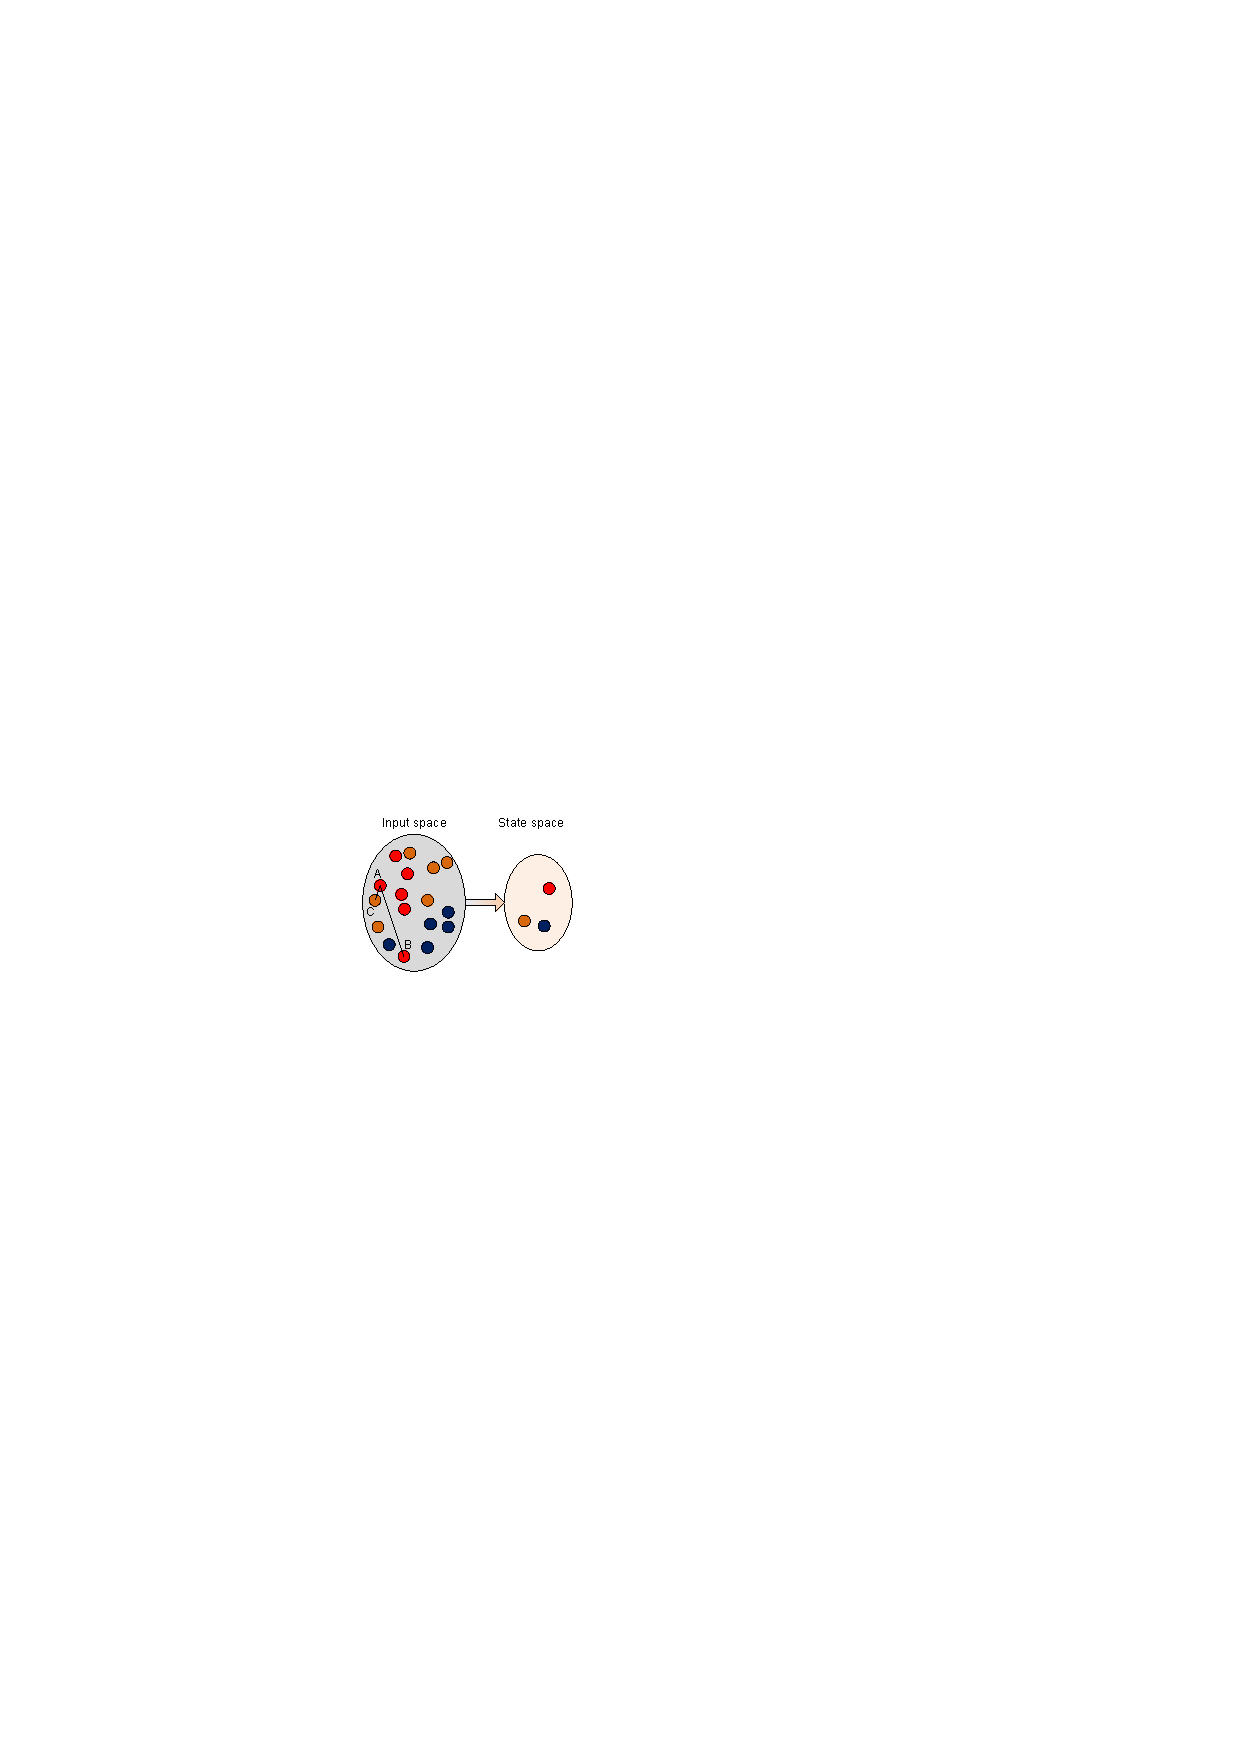
\includegraphics[width=0.5\textwidth]{figures/distance-illusion.pdf} 
\caption{An illusion for distance.}\label{distance-illusion}
\end{figure}

Based on the mapped bitmap vectors, the test case queue in the fuzzer is enhanced by assigning each test case with weight $W$ which is obtained from the distance between every two test cases. Whenever a new seed file is found, the distance between this seed file and all the other files in the queue will be measured to calculate $W$. Meanwhile, the weight of all the other files in the queue will be updated according to the distance to the new seed file. 

Rather than selecting the seed file that has the longest distance to the current seed file which is only a \emph{local optimum solution}, our search method selects the file that takes the longest average distance from all the other test cases as the next seed file. By doing this, we can achieve the \emph{global optimum solution} for this searching problem. The weight $W$ for test case $t_k$ is defined as follows:

\begin{center}
$W_k = \displaystyle\frac{1}{N} \sum_{i=0}^{N} D(t_i, t_k)$
\end{center}
where $D(t_i, t_k)$ denotes the distance between $t_i$ and $t_k$ based on the three distance measures mentioned before, and $N$ is the size of the test case queue. 

% Add memory coverage information
We also noticed that even two test cases have the same $W$ value, they can contribute different new paths. This is because code/path coverage is not the only criteria for testing, other runtime information, such as memory operations, can also be leveraged to prioritize test cases. So we enhanced the weigh $W$ with memory coverage to achieve better prioritization result. The enhanced weight $\hat{W_k}$ for test case $t_k$ is defined as the following formula, where $M(t_k)$ denotes the number of memory cells that $t_k$ covers in byte.
\begin{center}
$\hat{W_k} = \displaystyle M(t_k) + \frac{1}{N} \sum_{i=0}^{N} D(t_i, t_k)$
\end{center} 

\section{Selective branch query} 
Hybrid testing can help to reduce \textit{memory overhead} by 
limiting the number of states to an acceptable level. However, 
as mentioned in Section~\ref{sec:introduction}, symbolic pointers 
and loops will quickly generate lots of useless states that may 
not cover new code areas but bring serious performance overhead.

To address the large number of states forked from symbolic pointers, 
we propose a novel \textit{lazily concretization} of symbolic 
pointers which can not only reduce the number of states but also 
improve coverage. 
For symbolic loops, we introduce an optimization based on AFL's 
\textit{loop bucket} to control forking in symbolic loops. By 
doing this, execution can reach deeper code areas without 
generating lots of states. Both improvements will be discussed 
in the following sections.

\begin{figure}
\centering
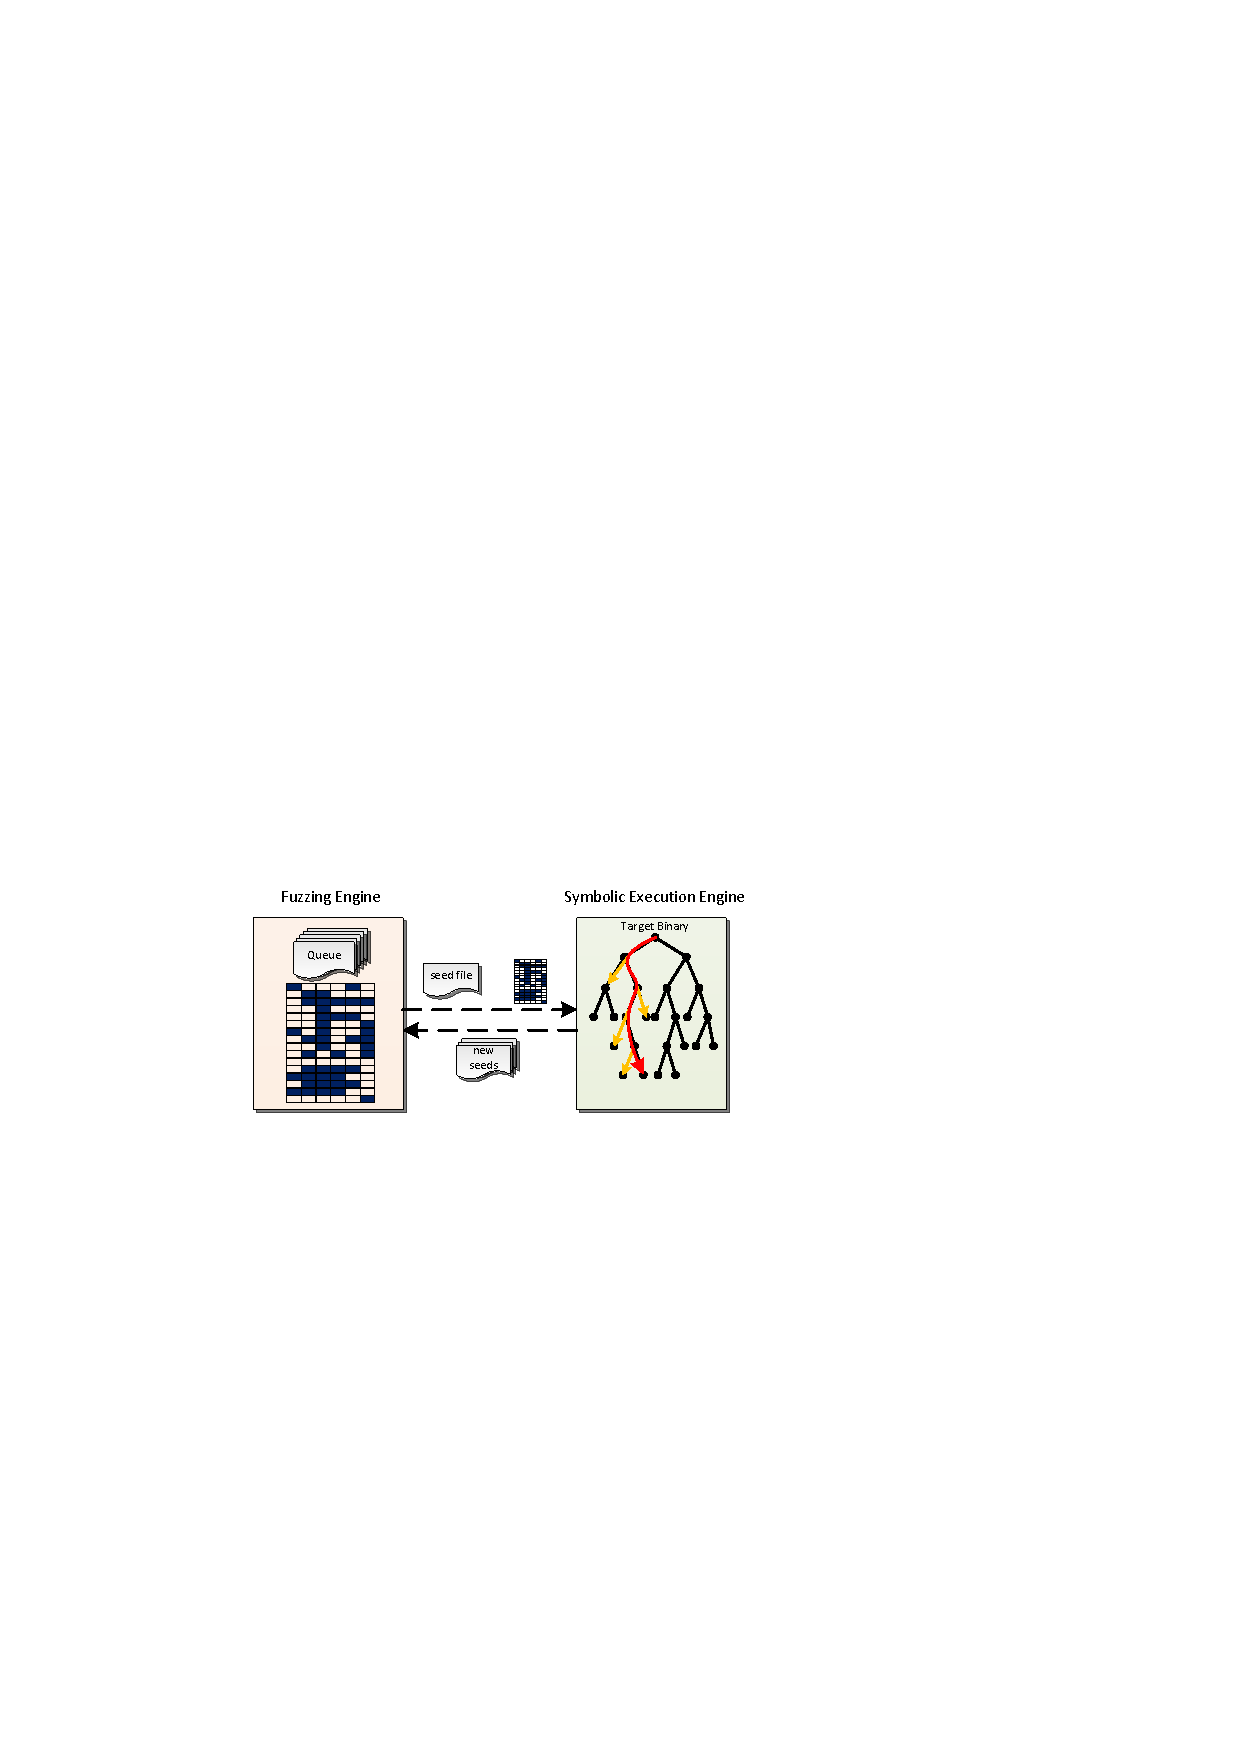
\includegraphics[width=0.5\textwidth]{figures/s2e-assist.pdf} 
\caption{Dynamic symbolic execution assisted fuzz testing. The 
	symbolic execution engine can help generate fresh seeds for 
	the fuzzing engine based on the seed files 	and the already 
	explored path information.}\label{s2e-assist}
\end{figure}

\subsection{Lazy Concretization of Symbolic Pointer}
The code snippet in Listing~\ref{RE-LCSP} shows the basic symbolic pointer 
problem in dynamic symbolic execution. The first parameter 
(i.e., \texttt{buf}) of function \texttt{looks\_ascii} points to memory 
that contains symbolic input data. The \texttt{nbytes} parameter is a 
concrete value that denotes the size of the memory buffer pointed by 
\texttt{buf}. \texttt{ubuf} is a shadow buffer which is used for further 
processing. 
Function \texttt{looks\_ascii} tries to determine whether each character 
of the symbolic input data appears in plain ASCII text, and returns 
immediately once a non-plain ASCII text character appears. 
The symbolic execution engine faces the symbolic pointer problem when executing 
the code at line 18 because \texttt{buf[i]} is from the symbolic input data. 
The memory range of \texttt{text\_chars[buf[i]]} spans from \texttt{\&text\_chars} 
to \texttt{\&text\_chars+255}. Since the binary executable loses the 
type information, the symbolic execution engine may need to explore all 256 possible
values for each \texttt{buf[i]} at the worst case. Meanwhile, the loop from line
17 to line 22 makes the trigger of the bug at line 26 even harder since more
states will be forked when \texttt{nbytes} is a larger one.
% Inaccurate expression for FSMM.
%Since \texttt{buf[i]} has 256 possible values (\textit{unsigned char}), 
%then the symbolic engine will fork state for each possible value (i.e., 
%fully symbolic memory model).
%This will cause the code at Line 18 to fork 
%$256^{nbytes}$ states, causing path explosion. The bug nested at line 26 
%will only be triggered when the states that satisfy the path condition 
%are scheduled for execution, which may never practically occur in the 
%face of path explosion. For example, suppose \texttt{nbytes} is 4, then 
%the worst case is that the bug can only be triggered after all 
%$256^4=4294967296$ states are scheduled.

There are different approaches for handling path explosion caused by
symbolic pointers. For example, treating memory address as \textbf{fully symbolic} 
enables the executor to reason about all possible values for symbolic pointer
\cite{song2008bitblaze, thakur2010directed, brumley2011bap, trtik2014symbolic}.
This can be achieved by either forking states or employing nested 
\textit{if-then-else} formulas which encode all possible values. 
However, since a symbolic address may pointer to any memory cell, fully symbolic
memory model fails to scale for real-world binary software. 
Some researches leverage the \textit{theories of arrays} to make fully symbolic 
memory model scalable \cite{cadar2006exe}\cite{cadar2008klee}. 
For example, KLEE \cite{cadar2008klee} forks states for values that reference 
different objects, and the \textit{theories of arrays} is leveraged within the same object.
However, since our target is to analyze binary executable whose object size of data structure is 
unavailable, the number of objects increases because each possible value may reference to a 
different object.
In contrast to reason about all possible values, a \textbf{partial symbolic} memory model has been proposed \cite{cha2012unleashing, avgerinos2014exploiting, Shoshitaishvili_firmalice-automatic}.  
The partial symbolic memory model tries to concretize all symbolic pointer write 
operation and treats symbolic pointer read operation using a fully 
symbolic memory model when contiguous interval of possible values is small enough.
However, if the possible values spans a large area, partial symbolic memory model
still needs to concretize the symbolic pointer which may lose some soundness paths.

%% Inaccurate description for fully and partial symbolic memory model.
%There are different approaches for handling path explosion caused by 
%symbolic pointers. For example, in the \textbf{fully symbolic memory model}, 
%each possible value of symbolic pointer will fork a corresponding state 
%\cite{song2008bitblaze, thakur2010directed, brumley2011bap, trtik2014symbolic}.
%In contrast, the \textit{address concretization} strategy will concretize 
%the pointer to a specific address \cite{godefroid2005dart, burnim2008heuristics}. 
%Obviously, the fully symbolic memory model may cause path explosion 
%(as mentioned before) and the address concretization may lose some 
%interesting paths. To mitigate the scalability problems of fully symbolic 
%memory model and the loss of interesting paths of address concretization, 
%a \textbf{partial symbolic memory model} has been proposed \cite{cha2012unleashing, avgerinos2014exploiting, Shoshitaishvili_firmalice-automatic}. The partial 
%symbolic memory model tries to concretize all symbolic pointer write 
%operation and treats all symbolic pointer read operation using a fully 
%symbolic memory model. However, because the instruction at line 18 is a 
%read operation, the partial symbolic memory model will still fork $256^{nbytes}$ states.

The \textit{lazy forking} strategy leveraged in S2E was proposed to avoid 
maintaining expensive symbolic pointers and ease the large number 
of states by forking \textit{pending states} in concolic 
execution \cite{chipounov2011s2e}. 
Consider a memory dereference instruction $I\in Inst$ in program $P$, 
suppose $I$ tries to access memory indexed by a symbolic expression 
$e_{addr}$.
Lazy forking treats such instruction $I$ as a conditional instruction 
and forks new states for $I$. It first evaluates the concrete value 
as $c_{addr}$, then it constructs an equal
expression $condition:= EQ(e_{addr}, c_{addr})$ 
which points $e_{addr}$ to this concrete value. Then it forks a 
new state $s_p=fork(s, ^\neg condition)$ which is labeled as a 
``pending state''. After that, each possible value of $e_{addr}$ 
will be exercised by systematically repeating this process. Even 
though lazy forking still needs to enumerate all possible values, 
it can avoid overhead by significantly reducing the total number 
of states that simultaneously exist in system. Here, 
the $condition$ is called a \textit{hard constraint} and 
$^\neg condition$ is called a \textit{soft constraint}.

For example, for the memory dereference instruction at line 18 
in Listing~\ref{RE-LCSP}, suppose the concrete value of 
\texttt{buf[i]} for $i\in[0,1,2,3]$ is `\texttt{A}'. 
In this case lazy forking will fork a new pending state and 
add the soft constraint $\texttt{buf[i]}\neq\texttt{`A'}$ to 
it. Meanwhile, the path constraint of the original state will 
be appended with the hard constraint $\texttt{buf[i]}=\texttt{`A'}$.
By doing this, the ``path explosion'' problem is postponed to a later moment.

However, the hard constraint may reduce the suffix feasible paths 
to a very small group. For example, suppose the address of a symbolic 
pointer can be expressed as $e_{addr}=f(v_1, v_2,\cdots, v_n)$, 
where $v_1, v_2,\cdots, v_n\in Var$ are variables of program $P$. 
Then expression $condition:= EQ(e_{addr}, c_{addr})$ will limit 
the current execution path only feasible when ($v_1, v_2,\cdots, v_n$) 
equals to ($c_1, c_2,\cdots, c_n$), where $c_i$ are the 
corresponding concrete values. 
Take the sample code in Listing~\ref{RE-LCSP}. The execution path 
to line 26 will be infeasible because the hard constraint limits 
the value of \texttt{buf[i]} ($i\in[0,1,2,3]$) to `\texttt{A}'. 
And the crash can only be triggered after enumerating all possible 
values for \texttt{buf[i]} ($i\in[0,1,2,3]$) in the worst case since
lazy forking still belongs to DFS state exploration strategy.
So even though lazy forking can ease the path explosion problem, 
it may still need to take longer time to trigger interesting paths. 
This will result in performance loss, because the symbolic 
execution engine will hold up the fuzzer. 

To mitigate this problem, we introduce a novel method 
\emph{lazy concretization of symbolic pointer} (LCSP) 
which is built on top of lazy forking. The detailed algorithm 
of LCSP is shown in Algorithm~\ref{LCSP}.


\lstinputlisting[label={RE-LCSP}, language=C,style=c,caption={A 
	motivating code derived from \texttt{file} in GNU Coreutils that contains symbolic pointer dereference at line 18.}, 
float=tp]{codes/real-eaxmple-LSP.c} 

Whenever the execution engine touches a symbolic pointer $e_{addr}$, it obtains 
the range of all possible values $\mathcal{R}$ by invoking function \texttt{getRange} 
in constraint solver. Then memory values $v$ within the range are dissolved
into buckets $\mathcal{B}=\langle v, addr\rangle$, where $v$ is the memory value; $addr$
is the set of memory cell's address whose memory value is $v$. 
After this, we reuse S2E's lazy forking method to pickup 
the buckets that contains the concrete value of this symbolic pointer.
For example, when executing the code at line 18 in Listing~\ref{RE-LCSP}, the range of 
the symbolic pointer is $\mathcal{R}=\texttt{\&text\_chars}+\{0, 1,\cdots, 255\}$.
By scanning the memory cells within $\mathcal{R}$, we can build 4 buckets, i.e., 

$\mathcal{B}_0=\{v=0| addr=[0,1,2,3,4,5,6,11,14,15,\cdots]\}$

$\mathcal{B}_1=\{v=1| addr=[7,8,9,10,12,13,\cdots]\}$

$\mathcal{B}_2=\{v=2| addr=[160,161\cdots, 253,254,255]\}$

$\mathcal{B}_3=\{v=3| addr=[128,129,130,\cdots,159]\}$

Since $e_{addr}$'s concrete value belongs to $\mathcal{B}_1$, we then
introduce a new symbolic variable $v_p$ into the engine and update current path constraint by adding expanded hard constraint $condition$ to it. 
$condition$ is descried as $P_\mathcal{B}\cap P_v\cap P_p$, where

$P_\mathcal{B}=\{\bigcup\limits_{i=0}^{Len_{addr}-1}e_{addr}=addr_i\}$;

$P_v=\{v_p=1\}$; 

$P_p=\{e_{addr}=\&\texttt{text\_chars}+0x41\}$.

During the following execution, all path conditions that related to the newly
introduced symbolic variable $v_p$ will be collected as pointer dereference constraint
$C_{pd}$.
This constraint is used to keep execution consistency.

\begin{algorithm}
 \LinesNumbered
  \caption{Lazy concretization of symbolic pointer}
  \label{LCSP}
  \KwIn{Current state $S$, pending states $S_P$, hard constraint $C_H$, 
  	    pointer dereference constraint $C_{pd}$.}
  \KwOut{Testcase $t_{lsp}$ if success.}
  $C_F = getFailedCondition()$\;
  % ignore cases that unrelated to symbolic pointer
  \If{$C_F$ \textbf{is not result from symbolic pointer}}
  {
  	return $null$\;
  }
  $offs = S.getInputOffset(C_F)$\;
  
  % Collect all possible bucket's addr to Solutions
  $extraCond\leftarrow True$\;
  \ForEach{$s_p$ in $S_P$}
  {
  	$off_{fork} = s_p$.getInputOffset($s_p$.forkCondition)\;
  	\If{$off_{fork}$ not in $offs$}
  	{continue\;}
  	$\mathcal{B}=s_p$.buckets\;
  	$e_{addr} = s_p$.getForkAddr()\;
  	% find all satisfied buckets
  	$\mathcal{B}_{sat}=s_p$.getSATBuckets($C_{pd}$, $\mathcal{B}$)\;
  	
  	% sieve real solutions out
  	$curExtraCond\leftarrow False$\;
  	\ForEach{$addr$ in $\mathcal{B}_{sat}$.addr}
  	{
      $s_{tmp} = S$.clone()\;
      $s_{tmp}$.getConditions().strip($C_H$)\;
      $s_{tmp}$.addConstraint($C_F$)\;
      $C_{new}\leftarrow \{e_{addr}=addr\}$\;
      $success = s_{tmp}$.evaluate($C_{new}$)\;
      \If{success}
      {$curExtraCond\leftarrow curExtraCond\cup C_{new}$\;}
  	}
  	$extraCond\leftarrow extraCond\cap curExtraCond$\;
  }
  
  $s_{tmp} = S$.clone()\;
  $s_{tmp}$.getConditions().strip($C_H$)\;
  $s_{tmp}$.getConditions().strip($C_{pd}$)\;
  $s_{tmp}$.addConstraint($extraCond$)\;
  
  $(success, t_{lsp}) = s_{tmp}$.generateTestcase()\;
  \If{$success$}
  {
    return $t_{lsp}$;
  }
  return $null$\;
\end{algorithm}

When performing lazy forking, all the states whose path constraints 
contain the soft constraints will be collected into \emph{Pending States}
as well as the buckets. 
These pending states are grouped by the program variables (e.g., each 
byte in an input file) that affect the corresponding soft constraint. 
They are also ordered along with the execution trace.
Then when the dynamic symbolic execution engine detects an infeasible 
branch due to hard constraints from symbolic pointer (line 3$\sim$5), 
the branch condition $C_F$ will be 
investigated to extract the program variables $offs$ (line 5).



Since we introduce new symbolic variable when dereferencing a symbolic pointer,
we need to make sure all conditions in $C_{pd}$ are satisfied so that the generated
test case can keep execution consistency.
Line 14 collects all satisfied buckets into $\mathcal{B}_{sat}$. The collect procedure
is light-weight since \texttt{getSATBuckets} only needs to evaluate $C_{pd}$
under each bucket's key (i.e.,$v$).
For each satisfied bucket, real solutions for current $e_{addr}$ are sieved out 
(line 16$\sim$25). This is achieved by evaluating each $addr$ in $\mathcal{B}_{sat}$
(line 20\&21). All $C_{new}$ evaluated as True will be collected together (line 22
$\sim$24). The $\cup$ in line 23 compacts consecutive $addr$s into a range expression.
For example, $\{e_addr=4\}$, $\{e_addr=5\}$ and $\{e_addr=6\}$ will be transformed to
$\{4<=e_addr<=6\}$.

By analyzing all pending states, the final extra condition $extraCond$ is constructed
(line 26).
After this, we remove $C_H$ and $C_{pd}$ from a newly cloned state $s_{tmp}$
from current state and append
the final extra condition to it (line 29$\sim$31). 
The reason why $C_{pd}$ is stripped is because it is already satisfied at line 14.
After appending all related conditions, the dynamic symbolic execution 
engine will try to generate a new test case (line 32), and once the 
generation successes, the test case $t_{lsp}$ will be sent to the 
fuzzer to find more paths.

For the code in Listing~\ref{RE-LCSP}, suppose \texttt{nbytes} is 5. 
Then when dynamic symbolic execution reaches line 24, there will be 
six states in the system: one execution state $S_0$ and five pending 
states ($P_0$, $P_1$, $P_2$, $P_3$, and $P_4$). $P_i$ is forked when 
dereferencing \texttt{buf[$i$]} at line 18. And pointer dereference
constraint $C_{pd}$ is $\{v_0=T\cap v_1=T\cap v_2=T\cap v_3=T\cap v_4=T\}$,
where $v_i$ is introduced for each symbolic pointer dereference at
line 18.

Because of the hard constraint, the four condition instructions at line 24
is infeasible. 
For example, for condition \texttt{ubuf[0]==`D'}, since line
18 introduces $\texttt{buf[0]=`A'}$, condition \texttt{ubuf[0]==`D'} cannot
be satisfied. LCSP first checks the input offset that results in this infeasible
condition and deals all pending states related to this offset. Based on this,
only $P_0$ is analyzed in order to break \texttt{ubuf[0]==`D'}. As mentioned before,
there are four buckets for $P_0$, i.e., $\mathcal{B}_0$, $\mathcal{B}_1$, $\mathcal{B}_2$,
$\mathcal{B}_3$. Then \texttt{getSATBuckets} verifies keys for all these four buckets 
to sieve the feasible ones. In this example, $\mathcal{B}_{sat}=\{\mathcal{B}_1\}$ since
$v_0=T$ in $C_{pd}$ must be satisfied. 

Then from line 16 to line 25 in Algorithm~\ref{LCSP} evaluates each $addr$ in $\mathcal{B}_1$ to build the final extra condition. The final constructed extra
condition for \texttt{ubuf[0]==`D'} in this example is $extraCond=\{\texttt{buf[0]=`D'}\}$.
This $extraCond$ keeps not only $C_F$ but also $C_{pd}$ be satisfied.
Then LCSP fixes current path condition by stripping unrelated conditions and adding
$\{\texttt{buf[0]=`D'}\}$ to it. After this, it invokes constraint solver to 
generate a fresh test case. Here, after breaking condition \texttt{ubuf[0]==`D'}, the 
generated test case is \texttt{DAAAA}. This test case will be sent to the fuzzer and the
remained three conditions at line 24 will be solved in the same way. Thus, based on this algorithm, we can generate at least one fresh test case 
that satisfies the branch condition whenever a branch is infeasible 
because of lazy forking. 

%Then path constraint for each states is shown in Table~\ref{table:path-conditions}.
%
%\begin{table}[!b]
%\processtable{Path Constraint for each state when reaching line 24 in Listing~\ref{RE-LCSP}.
%	\label{table:path-conditions}}
%{\begin{tabular*}{20pc}{@{\extracolsep{\fill}}lccccc@{}}\toprule
%State  & buf[0] & buf[1] & buf[2] & buf[3] & buf[4]\\ 
%\midrule
%		$S_0$  &  $=$ `A' & $=$ `A' & $=$ `A' & $=$ `A' & $=$ `A' \\
%		$P_0$  &  $\neq$ `A' & N/A & N/A & N/A & N/A \\
%		$P_1$  &  $=$ `A' & $\neq$ `A' & N/A & N/A & N/A\\
%		$P_2$  &  $=$ `A' & $=$ `A' & $\neq$ `A' & N/A & N/A \\
%		$P_3$  &  $=$ `A' & $=$ `A' & $=$ `A' & $\neq$ `A' & N/A \\
%		$P_4$  &  $=$ `A' & $=$ `A' & $=$ `A' & $=$ `A' & $\neq$ `A' \\
%\botrule
%\end{tabular*}}{}
%\end{table}
%
%The hard constraint for $S_0$ is $C_{H}\leftarrow$ \{\texttt{buf[0]$=$`A'\& buf[1]$=$`A'\&buf[2]$=$`A'\&buf[3]$=$`A'\&buf[4]$=$`A'}\}. 
%Because of $C_{H}$, the branch condition at line 24\&25 ($C_{F}\leftarrow$ \{\texttt{buf[0]$=$`D'\&buf[1]$=$`E'\&buf[2]$=$`A'\&buf[3]$=$`D'}\}) will 
%be infeasible.
%Based on \textit{LCSP}, the path conditions of $S_0$ (except for the related 
%hard conditions) will be append to each pending state to generate new test case. 
%After stripping the related hard conditions, the \textit{Conditions} at line 
%6 in Listing~\ref{LCSP} will be $\texttt{buf[4]}=\texttt{`A'}$. 
%Then \textit{Conditions} will be added to each pending state. For example, 
%the path constraint of $P_0$ after adding such conditions will be 
%\{\texttt{buf[0]$\neq$`A' \& buf[4]$=$`A' \& buf[0]$=$`D' \& buf[1]$=$`E' \& buf[2]$=$`A' \& buf[3]$=$`D'}\}. After solving this path constraint, we can successfully 
%generate a test case that satisfies the condition at line 24\&25 and 
%triggers the bug at line 26. 
%
%An interesting point in our example is that $P_1$, $P_2$, $P_3$, and 
%$P_4$ cannot successfully trigger this bug. This does not mean that 
%these states are useless. 
%For example, if the condition at line 24\&25 is 
%\{\texttt{buf[0]$=$`A' \& buf[1]$=$`B' \& buf[2]$=$`C' \& buf[3]$=$`D'}\}, 
%then $P_1$ can successfully generate a corresponding test case 
%that triggers the bug.


%% Remove this proof since the consistency is kept by the constraint solver.
%But we still need to prove this test case 
%will steer the program to execute the same path with the original 
%state and then covers the branch that fails in the original state. 
%A quick execution consistency proof is explained as follows:
%
%Let $P_A$ be the execution path of a state $A$ which contains 
%the following branches:
%\begin{center}
%$P_A:(B_0) \rightarrow (B_1) \rightarrow (B_2) \rightarrow 
%(B_3) \rightarrow (B_4) \rightarrow (B_5) \rightarrow (B_6) \rightarrow (B_u)$
%\end{center}
%
%\noindent where $B_i$ refers to the $i$-th branch, and $B_u$ 
%denotes the infeasible branch that because of the extra hard constraint.
%And its path constraint is:
%\begin{center}
%$PC_A\leftarrow \displaystyle \bigcap\limits_{i=0}^{6} CB_i \cap CB_u$
%\end{center}
%, where the $CB_i$ denotes the path condition at branch $B_i$.
%
%Assume that the hard constraint is $var=0xAB$ which is originated 
%from lazy forking from $B_1$. 
%We also assume that the branch conditions at $B_3$ and $B_5$ are 
%also affected by $var$; state $B$ is the corresponding pending state 
%forked from $B_1$, and its path constraint is:
%\begin{center}
%$PC_B\leftarrow\displaystyle CB_0 \cap ^\neg CB_1$
%\end{center}
%, where $^\neg CB_1$ is the soft constraint.
%
%Then, according to the \textit{LCSP} algorithm in Listing~\ref{LCSP}, 
%when state $A$ detects the infeasible branch $B_u$ because of hard 
%constrain, all the related constraints except the hard constraint 
%of state $A$ will be added to state $B$. After that, the path 
%constraint of state $B$ will be:
%
%\begin{center}
%$PC_B\leftarrow\displaystyle CB_0 \cap ^\neg CB_1 
%\cap (\bigcap\limits_{i=0,i \neq 1}^{6} CB_i) \cap ^\neg CB_u$
%\end{center}
%where $^\neg CB_u $ is the branch condition we want to cover 
%and $\bigcap_{i=0,i \neq 1}^{6} CB_i$ is the conditions from 
%state $A$ after stripping the hard constraint.
%
%We need to prove the following formula:
%
%\begin{center}
%$\mathbb{Z}=\{var\arrowvert PC_B(var) = True\} \neq \emptyset$
%\end{center}
%
%As there are only two branches before $B_u$ that depend on $var$, 
%the expression $PC_B$ can be simplified to:
%\begin{center}
%$PC_B\leftarrow^\neg CB_u \cap ^\neg CB_1 \cap CB_3 \cap CB_5$
%\end{center}
%
%There are two possible cases for $CB_3 \cap CB_5$:
%\begin{center}
%case1: $CB_3 \cap CB_5 = (var = 0xAB)$
%
%case2: $CB_3 \cap CB_5 \neq (var = 0xAB)$
%\end{center}
%
%Under the first case, the path to $B_u$ is only feasible when 
%$var$ equals to $0xAB$. So the edge $^\neg B_u$ can never be 
%satisfied (i.e., \emph{dead code}) because $(var = 0xAB) \subseteq CB_u$. 
%For the second case, there must be at least one feasible solution 
%for $var$ that satisfies the soft constraint $^\neg CB_1$, so 
%$^\neg CB_1 \cap \bigcap_{i=0,i \neq 1}^{6} CB_i$ can be evaluated 
%to $True$ for some specified values of $var$. This has proved that 
%there must be at least one test case under $PC_B$ that can steer 
%the program to the infeasible branch $B_u$.
%
%Similarly, for branch condition $B_u$, there are also two possible cases:
%\begin{center}
%case1: $\displaystyle ^\neg CB_1 \cap \bigcap\limits_{i=0,i\neq 1}^6 CB_i \subseteq CB_u$
%
%case2: $\displaystyle ^\neg CB_1 \cap \bigcap\limits_{i=0,i\neq 1}^6 CB_i \nsubseteq CB_u$
%\end{center}
%
%The first case, which can also be expressed as 
%$^\neg CB_u \cap ^\neg CB_1 \cap \bigcap_{i=0,i\neq 1}^6 CB_i = \emptyset$, 
%is the case of \emph{dead code}. And the second case can be transformed into:
%\begin{center}
%$\displaystyle ^\neg CB_u \cap ^\neg CB_1 \cap \bigcap\limits_{i=0,i\neq 1}^6 CB_i \neq \emptyset \implies \mathbb{Z} = \{var\arrowvert PC_B(var) = True\} \neq \emptyset$
%\end{center}
%
%\noindent which means there must be at least one feasible value 
%that satisfies the false branch of $B_u$.
%
%So above all, we can draw a conclusion that our \emph{LCSP} algorithm 
%can keep the execution consistency when $^\neg B_u$ is not dead code.

\subsection{Optimization for Symbolic Loop}
Symbolic loop, whose loop control variable depends on symbolic data, 
is another common cause of path explosion since its loop times may 
range from 0 to infinite theoretically. 
Even though the hybrid testing method can ease path explosion, the 
states forked from a symbolic loop will quickly force the number of 
states to increase to the budget's upper bound. 

\lstinputlisting[label={RE-SLB}, language=C,style=c,caption={A motivating 
	example to demonstrate path explosion raised by symbolic loops.}]
{codes/example-SLB.c} 

The code snippet in Listing~\ref{RE-SLB} demonstrates this problem. 
Function \texttt{verify\_packet} reads the \texttt{length} of the 
raw data from the \texttt{packet} at line 4.
 Then from Line 6 to 10, it investigates each bytes in the raw data 
 to determine whether there exists the ending descriptor 
 (i.e., \texttt{0xFF}) through a loop structure. 
 Suppose we have a test case from the seed queue of 
 the fuzzer and its \texttt{length} is \texttt{0xAA}, 
 then the symbolic loop 
 from line 6 to 10 (\texttt{length} is symbolic) 
 will result in path explosion.
 Because the possible value of \texttt{length} is in the 
 range of [0, $2^{32}-1$], $2^{32}$ states will be forked from 
 line 6 in the worst case. 
Most of the forked states from line 6 may not contribute 
to any new code coverage but only bring performance overhead.
It is therefore important to also handle symbolic loops. 

AEG \cite{Avgerinos:2014:AEG:2556647.2560219} proposes \emph{loop exhaustion}
search strategy to handle symbolic loops. It tries to execute the loop as many
times as possible. Since it focuses only on maximizing the loop iterations which
may fork lots of states, it thus may stuck the fuzzer from exploring more paths 
in our hybrid testing framework.

A \textit{boundary state prioritization} method has been proposed recently
to ease the path explosion problem due to symbolic loops.
The key idea of this prioritization is to defer the analysis of 
uninteresting states based on the likelihood of a security vulnerability \cite{cab-fuzz}. 
Specifically, it focuses only on three types of states for a symbolic 
loop: \textit{no loop execution}, \textit{single loop execution}, and 
\textit{the largest number of loop executions}.
The author implemented such a strategy within S2E \cite{chipounov2011s2e} 
and produced a vulnerability detection tool \textit{CAB-Fuzz}.
It successfully found 21 undisclosed unique crashes in Windows 7 and 
Windows Server 2008 \cite{cab-fuzz}.
 
We extend this boundary state prioritization method by integrating it 
with the \emph{Loop Bucket} mechanism employed in AFL \cite{online:afl} 
to achieve better performance on finding vulnerabilities.
AFL utilizes \emph{Loop Bucket} to avoid collecting too many test cases 
which only affect the loop times into the seed queue \cite{online:afl}. 
It groups the loop times into 8 different buckets, i.e., 
[1, 2, 3, 4-7, 8-15, 16-31, 32-127, 128+]. Only changes that occur 
between different buckets will be regarded as new behaviors. 
Based on this idea, we proposed a \textit{Symbolic Loop Bucket} (SLB) 
to handle the symbolic loop when performing hybrid testing. The 
algorithm of SLB is described in Algorithm~\ref{SLB}.

Loops are extracted from the target program by static analysis. 
These loops will be configured in the dynamic symbolic execution 
engine to help it recognize loops in runtime. All the symbolic loops 
can be distinguished from the others by checking whether the loop 
exit condition is affected by symbolic data or not (line 1$\sim$3). 
For the edge belongs to symbolic loop, the uncovered loop buckets 
for this loop will be obtained by analyzing the \textit{Bitmap} 
mentioned before (line 5). 
In already covered loop buckets, the program will loop for one more 
time without forking new state (line 16\&17). Once an uncovered bucket 
is reached, the corresponding test case will be generated and then 
this uncovered bucket will be removed from the uncovered loop buckets 
to avoid generating multiple test cases (line 7$\sim$12). After 
generating test cases for all the uncovered buckets, the loop will 
be prohibited from being executed for more times. This can make sure 
that all the loop buckets will be covered without causing path explosion.

\begin{algorithm}
  \LinesNumbered
  \caption{Symbolic loop bucket.}
  \label{SLB}
  \KwIn{Configured Loops $L$, Current Edge $CE$ and Bitmap $B_p$}
  \KwOut{Generated test cases $t_{slb}$}  
  \If{not $IsaLoopCycleEdge(L,CE)$ or not $IsaSymLoop(CE)$}
  {
    return;
  }
  $loopTimes$ = 1\;
  $UBs$ = $ParseUncoveredBuckets(B_p)$\;
  \While{TRUE}
  {
    \ForEach{$ub$ in $UBs$}
    {
      \If{$loopTimes$ within $ub$}
      {
        $t_{slb}.add(GenerateTestcase())$\;
        $UBs$.$remove(ub)$\;
      }
    }
    \eIf{$UBs$ is $null$}
    {
      return $t_{lsb}$\;
    }{
      $ExecuteOneCycle()$\;
      $loopTimes += 1$\;
    }
  }
\end{algorithm}  

For the symbolic loop in Listing~\ref{RE-SLB}. Suppose previous 
test cases have covered the buckets of [1], [2], [3], and [4-7]. 
Then \textit{UBs} at line 5 in Algorithm~\ref{SLB} will consist of 
[8-15], [16-31], [32-127], and [128+]. 
$\textit{loopTimes}=[1, 2, \cdots, 7]$ will not fork any new states 
according to line 15 to 18. Then once the \textit{loopTimes} reaches 
8 which belongs to an uncovered bucket [8-15], the engine forks a 
new state,  generates the corresponding the test case, and removes 
bucket [8-15] from \textit{UBs}. The execution engines will not 
fork new states until \textit{loopTimes} reaches 16, 32 and 128. 
Once all the loop buckets are covered, the forking in this 
symbolic loop will be disabled. It will continue cycling until 
\textit{loopTimes} reaches the concrete value of \texttt{length} 
(i.e., \texttt{0xAA}) and then exercise deeper code areas.


\section{Implementation}
\prototype is built on top of AFL \cite{online:afl}, a popular 
state-of-the-art genetic fuzzing framework, and the S2E symbolic 
execution platform \cite{chipounov2011s2e}. S2E is a dynamic 
binary analysis platform which utilizes selective symbolic execution 
to analyze whole software stacks at runtime. S2E reuses parts of 
the QEMU virtual machine \cite{bellard2005qemu}, the KLEE symbolic 
execution engine \cite{cadar2008klee} and the LLVM 
toolchains \cite{lattner2004llvm}.

Our implementation consists of two main components, namely
\emph{Symbolic Path Finder (SPF)} and \emph{Seacher}. The \emph{SPF}
component is leveraged to help the fuzzer dive into deeper code areas
that are guarded by complex path constraints. Techniques to handle the
\textit{path explosion} problem raised by symbolic pointers and loops
are implemented inside of \emph{SPF}. The \emph{Searcher} is designed
to assign more mutation energy to the promising seeds based on the weight
value obtained by distance based seed selection method. 
By doing this, the fuzzer will reach previously
untouched more code areas as soon as possible in a given time budget.



\section{Evaluation}
In the experimental evaluation part, we address the following 
research questions:
\begin{itemize}
\setlength{\itemsep}{0pt}
\item {\textbf{RQ1:} Can \prototype discover more deeper bugs?}
\item {\textbf{RQ2:} Can distance based seed selection method 
	improve performance of path discovery?}
\item {\textbf{RQ3:} How does each component contribute to 
	path discovery?}
\end{itemize}

More specifically, RQ1 investigates the bug discovery ability of 
\prototype and compares the results with other vulnerability 
detection tools including fuzz testing and dynamic symbolic execution. 
For RQ2 and RQ3, we choose to use AFL's \textit{unique paths} as performance evaluation criterion since it is a key factor to reflect the 
performance of a path-based program testing tool.
RQ2 evaluates distance based seed selection on several 
real-world programs to see whether our method can discover more 
unique paths than the state-of-the-art fuzzer: AFL. RQ3 evaluates 
the overall unique path discovery performance of \prototype and 
investigates the performance contribution of each isolated 
component (i.e. \textit{SPF} and \textit{Searcher}).
Evaluations were conducted on a server equipped
with an Intel Xeon CPU E7-2850 @ 2.0GHz with
20 cores and 128 GB RAM, running Linux Ubuntu 14.04.

\subsection{Vulnerability Detection (RQ1)}
We evaluated the bug discovery ability of our method with two 
different benchmarks and some real world software. The first 
benchmark is a demo program which is named as \emph{CommonMB}. 
The second benchmark is \emph{LAVA}, which was released in 2016 
to test different vulnerability discovery tools \cite{dolan2016lava}. 
In the following sections, we are going to introduce the 
two benchmarks, and discuss the testing results of \prototype
as well as other off-the-shelf vulnerability discovery tools 
(LibFuzzer \cite{libfuzzer}, AFL, KLEE, S2E, and VUzzer) in detail.

\subsubsection{CommonMB}
\noindent The \emph{CommonMB} benchmark is a demo program which contains 
9 different memory error bugs. These bugs can be triggered only when 
feeding the program with specifically crafted input. There are four 
different kinds of functions in this benchmark, i.e., 2 compare-style 
functions, 3 math-style functions, 2 checksum-style functions and 2 
logic-style functions. The compare functions contains bugs that can 
only be triggered when the values of specific parts of the input equal 
to specific constant immediate numbers; the bugs in math functions 
can be triggered when the results of math operation on some specific 
parts of the input equal to specific constant immediate numbers; the 
checksum related bugs can only be triggered when the input data 
successfully goes through the checksum checking points; and the logic 
bugs utilize two simple logical games (maze and semi-sudoku) as the 
constraints for triggering the bugs, which means the bugs can only be 
triggered when the testing engine successfully solves the games. We 
released \emph{CommonMB} benchmark at \texttt{https://github.com/Epeius/CommonMB.git}.

The bugs in \emph{CommonMB} benchmark represent the common bug conditions 
in real-world programs. For example, compare-style bugs denote the bugs 
that depend on some specific/interesting values in the program; 
checksum-style bugs stands for the bugs whose inputs are well-formatted, 
such as PNG file.
So evaluating a vulnerability detection tool on such a benchmark can 
reflect its ability of discovering bugs in real world programs.

Table~\ref{CommonMB-results-detail} shows the overall results of 
different vulnerability discovery tools as well as \prototype 
with same test environment (10 cores and 12 hours).
% Explain the result like that cmp-style vulnerabiities are easy to find
We can see that all these tools have successfully triggered the 
two compare-style bugs (i.e., \textit{cmp16} and \textit{cmp32}). 
This is because there two functions are in the shallow surface of 
this benchmark and the conditions to trigger the bugs are simpler 
than the others.  

% Explain the result, for example, why add32 cannot be found by KLEE...
Fuzz testing tools discovered few math-bugs than symbolic execution 
tools in average.
For example, AFL discovered the \textit{add16} and LibFuzzer triggered 
one more bug (i.e., \textit{add32}). And these two fuzzer both failed 
to uncover the bug that guarded by complex mathematic operations. 
All tools that leverage symbolic execution except KLEE successfully 
triggered all these three bugs since symbolic execution is good at 
solving such corner cases. One interesting point in this table is that 
KLEE failed to trigger \textit{add32} and \textit{complex} bugs. 
This is because KLEE forks too many states in checksum functions 
which raise the serious path explosion problem. 

S2E provides function models for basic functions that may fork too 
many states, like \texttt{strcpy}, \texttt{strcat}, \texttt{crc16},
 and \texttt{crc32}. Based on these models, S2E and \prototype 
 discovered the two bugs that related to checksum successfully 
 (note that this does not mean S2E can break these checksum functions). 

Logic-style vulnerabilities are difficult for all tools to uncover 
because the number of states will be infinite in the worse case.
For example, when solving a maze, the possible oscillation between 
two opposite steps (such as step forward and step backward) 
will stop the engine from finding new paths.
With the help of our seed selection method, \prototype selected 
the seed file with the maximum average distance to schedule. 
Since this distance metric tries to maximize the memory coverage, 
\prototype successfully triggered the bug after covering all 
the memory access to the maze array. 
% Explain why the sudodu is so hard to touch
However, our \prototype failed to trigger the bug in \textit{sudoku}. 
This is because different seed files of the \textit{sudoku} have no 
significant differences (i.e., no more code/branch and memory coverage), 
which confuses our seed selection method.

\begin{table*}[!t]
\processtable{Evaluation results on \textit{CommonMB} in detail.
	\label{CommonMB-results-detail}}
{\begin{tabular*}{20pc}{cccccccccccc}\toprule
	&& \multicolumn{2}{c}{CMP}  & \multicolumn{3}{c}{MATH} & \multicolumn{2}{c}{CHECKSUM} 
	& 	\multicolumn{2}{c}{LOGIC} & \\ 
	    Tool & version & cmp16 & cmp32 & add16 & add32 & complex & crc16 & 
	    crc32 & maze & sudoku & Total Crashes (\#) \\
\midrule
		AFL 		& 2.52b	& Y & Y & Y & N & N & N & N & N & N & 3 \\
		LibFuzzer	& llvm 3.8	& Y & Y & Y & Y & N & N & N & N & N & 4\\
		KLEE		& 1.4.0	& Y & Y & Y & N & N & N & N & N & N & 3\\
		S2E			& 2.0	& Y & Y & Y & Y & Y & Y & Y & N & N & 7\\
		\prototype	& 0.1	& Y & Y & Y & Y & Y & Y & Y & Y & N & 8\\
\botrule
\end{tabular*}}{}
\end{table*}

\subsubsection{LAVA Benchmark}
In 2016, Dolan-Gavitt et.al. developed a technique, namely LAVA, to 
automatically inject secure-related bugs into some Linux utilities for 
evaluating the bug-finding tools \cite{dolan2016lava}. These bugs are 
all hard-to-reach memory errors. In the paper of LAVA, the authors describe 
their results on the evaluation of coverage based fuzz testing, an SAT-based 
approach on the benchmark. The LAVA benchmark has two corpus sets, 
i.e., \textit{LAVA-1} and \textit{LAVA-M}.

\textit{LAVA-1} injected 69 different bugs into the \texttt{file} program 
in Linux CoreUtils. There are two types of buffer overflow vulnerabilities 
were injected, one is \emph{Range} and the other one is 
\emph{Knob-and-trigger (KT)}. The Range style bugs are triggered if the 
magic value is in some range and also check the value to determine how much 
to overflow. And in the KT bug, two bytes in the input are checked against 
a magic value to determine if the overflow will happen and another two bytes 
determine how much to overflow. Both the two types of bugs were designed to 
mirror real bug patterns which can be used to evaluate the ability of 
bug-finding tools. Compared \textit{LAVA-1}, which injected only one bug 
in the program, \textit{LAVA-M} injected more than one bug into four 
different programs in CoreUtils that took file input: \texttt{base64}, 
\texttt{md5sum}, \texttt{uniq}, and \texttt{who}, so \textit{LAVA-M} is a 
better benchmark to evaluate the vulnerability discovery tools that are 
designed to work for a long time on programs that may contain multiple bugs.

\begin{table}[!b]
\processtable{Evaluation results on \textit{LAVA-1}\label{LAVA-1}}
{\begin{tabular*}{20pc}{@{\extracolsep{\fill}}ccccccc@{\extracolsep{\fill}}}\toprule
& $2^0$ & $2^7$  & $2^{14}$ & $2^{21}$ & $2^{28}$ & KT \\
	      Tool   & (12 bugs) & (10 bugs) & (11 bugs) & (14 bugs) & (12 bugs) & (10 bugs)\\
\midrule
		FUZZER 		& 0   & 0   & 1    & 11    & 9     & 2  \\
		SES	        & 1   & 0   & 1    & 3     & 0     & 1  \\
		AFL		    & 0   & 0   & 2    & 10    & 9     & 1   \\
		S2E			& 3   & 2   & 3    & 4     & 3     & 2   \\
		\prototype	& 10  & 10  & 11   & 13    & 11    & 7   \\
\botrule
\end{tabular*}}{}
\end{table}

Table~\ref{LAVA-1} summarized the results of bug finding evaluation on 
\textit{LAVA-1} from the LAVA paper as well as some popular off-the-shelf 
tools (AFL and S2E). The maximum testing time for each bug was five hours. 
From this table, we can see that the \textbf{FUZZER} and \textbf{SES} 
mentioned in the paper only found 23 bugs and 6 bugs respectively in total. 
AFL found fewer paths than S2E in the small ranges ($2^0$, $2^7$ and $2^{14}$) 
but it outperformed S2E in larger ranges. 

\prototype discovered 62 bugs which was much more than the FUZZER and the 
SES tools separately. In particular, we triggered all the bugs in $2^7$ and 
$2^{14}$ ranges. And also found most of the KT bugs (70\%) which cannot be 
touched effectively by the FUZZER and SES tools. 

Table~\ref{LAVA-M} describes the evaluation results on LAVA-M of the FUZZER 
and SES which are mentioned in the LAVA paper. We also listed the results 
of VUzzer and \prototype in this table. 
\begin{table}[!b]
\processtable{Evaluation results on \textit{LAVA-M}\label{LAVA-M}}
{\begin{tabular*}{20pc}{@{\extracolsep{\fill}}cccccc@{}}\toprule
	     & \texttt{base64} & \texttt{md5sum} & \texttt{uniq} & \texttt{who} &   \\
	     Tool    & (44 bugs) & (57 bugs) & (28 bugs) & (2136 bugs) &  Total\\
\midrule
		FUZZER 		& 7  & 2  & 7    & 0   & 16  \\
		SES	        & 9  & 0  & 0    & 18  & 27  \\
		VUzzer		& 17 & 1* & 27   & 50  & 95 \\
		\prototype	& 37 & 29 & 28   & 203 & 297 \\
\botrule
\end{tabular*}}{}
\end{table}


As mentioned in the LAVA paper, SES cannot find any bugs in \texttt{uniq} and 
\texttt{md5sum}. And the reasons are the control flow is too unconstrained in 
\texttt{uniq} and SES failed to execute any code past the first instance of 
the hash function. Because our symbolic execution is driven by a concrete seed 
input, these two problems will be eased to a large extent, leading to the 
discovery of more bugs. Particularly, for program \texttt{md5sum}, VUzzer can 
only trigger one bug because it fails to get through the first crash to parse 
more of any input, whereas \prototype successfully triggered 29 bugs in 
\texttt{md5sum}.

\subsubsection{Real-World Programs}
We selected several real world programs to evaluate the ability of unknown bug 
discovery of our system. The input types of this dataset cover ELF binary, 
multi-media, image, and packet capture. In order to demonstrate the efficiency 
of our system, we also compared our results with AFL and VUzzer. We ran each
 program under the same testing environment with one fuzzing node for 24 hours. 

Table~\ref{zero-days} shows the results of our testing. 
From the table we can see that during 24 hours, \prototype triggered 403 
unique crashes in the dataset which outperformed vanilla AFL (181 unique crashes) 
and VUzzer (192 unique crashes). 
We can also derive from this table that our method gains little for \texttt{mp3gain} 
and \texttt{madplay}. This is because our symbolic execution engine does not support 
the float number operation when handing MPEG/WAV format (for example, all the 
writing operation to \texttt{XMM} registers will be concretized). This concretization 
lost some interesting paths and made less contribution to bug finding(only 2 more 
bugs for \texttt{mp3gain} and 1 more bug for \texttt{madplay}). 
This also explains the phenomena that VUzzer found more bugs in \texttt{mp3gain} 
than \prototype. 
It is interesting that AFL detected 15 more bugs in \texttt{elfparser} than VUzzer. 
This is because the fork server method leveraged in AFL enables the fuzzer can 
execute 51.6x more test cases than VUzzer in the same time, which can also increase 
the probability of finding bugs.

\begin{table*}[!t]
\processtable{Performance of our method VS. AFL \& VUzzer on unknown crashes.\label{zero-days}}
{\begin{tabular}{lccccccc}\toprule
	& & \multicolumn{2}{c}{\prototype} & \multicolumn{2}{c}{AFL} & \multicolumn{2}{c}{VUzzer}\\
		    Program & Input Type & Crashes (\#) & Executed (\#)& 
		    Crashes (\#) & Executed  (\#) & Crashes (\#) & Executed (\#) \\
\midrule
\texttt{elfparser}  & ELF	& 60 &   1.1M & 48   & 1.0M   & 33 & 19.0K    \\
		\texttt{distorm}    & ELF    & 13 &   16.2M   & 0   & 15.7M    & 3 & 93.1K    \\
		\texttt{mp3gain}*   & MPEG	& 43 &   11.3M  & 41  &  11.7M   & 46 &  79.3K  \\
		\texttt{madplay}*   & WAV	& 55 &   15.9M  & 54  & 14.3M    & 52 & 88.7K   \\
		\texttt{optipng}    & PNG    & 49 &   9.5M & 15  &  10.1M   & 32 & 54.1K   \\
		\texttt{tstat}      & PCAP   & 183&   6.4M & 23 &  6.2M   & 26 & 48.5K   \\
		\midrule
		Total      &        & 403   &  & 181 &  & 192 &\\
\botrule
\end{tabular}}{}
\end{table*}

\subsection{Coverage Performance (RQ2)}\label{sec:RQ2}
Our benchmark for coverage performance evaluation consists of 8 real-world binary 
programs, and the input file formats of our benchmark cover a range of types such 
as executables, images, archives and network packets.

To set the baseline of coverage performance, we utilized the state-of-the-art 
coverage based fuzzer AFL \cite{online:afl} and configured it to run under 
\textit{binary-testing} (i.e., option `-Q' is turned on) mode with one 
single work node.
 We collected and compared \textbf{the number of unique paths} found by 
 AFL and our distance based seed selection method.
 Then we select the most effective distance metric for 
 subsection~\ref{sec:RQ3}.
 All the evaluations lasted for 24 hours.

The evaluation results were shown in Table~\ref{PD-8samples}. We have 
investigated the three distance measures mentioned before (i.e., EU, CS, 
and JI) as well as the original seed selection strategy (Order) from 
vanilla AFL which selects test case in the seed queue one by one.
From this table, we can see that by prioritizing the mutation orders of 
seeds, the fuzzer can touch more unique paths in average.
 More clearly, Figure~\ref{path-detail}(a) shows the normalized unique 
 paths to vanilla AFL (i.e., orderly selection) for these 8 programs 
 based on the results in Table~\ref{PD-8samples}.
\begin{table}[!b]
\processtable{Number of unique paths discoverd for 8 sample programs\label{PD-8samples}}
{\begin{tabular*}{20pc}{@{\extracolsep{\fill}}lrrrr@{}}\toprule
	     Program  & Order\# & EU\# & CS\# & JI\# \\
\midrule
		\texttt{readelf}  &    2753 & 4595 & 5314 & 5062 \\
		 \texttt{djpeg }  &    2802 & 3020 & 4198 & 3390 \\
		\texttt{objdump} &    1755 & 2200 & 2960 & 2133 \\
		 \texttt{gzip }  &    1440 & 1564 & 1754 & 1588 \\
		 \texttt{ffmpeg}  &    5022 & 5993 & 6181 & 5801 \\
		\texttt{tcpdump}  &    3399 & 3673 & 4267 & 2950 \\
		\texttt{capstone} &    5626 & 6008 & 6066 & 5873 \\
		\texttt{gif2png}  &     912 &  981 & 1100 &  997 \\ 
\botrule
\end{tabular*}}{}
\end{table}


From Figure~\ref{path-detail}(a), we can see that both EU and CS metrics 
can outperform vanilla AFL on discovering unique paths for all programs 
in our benchmark. However, the average performance gain of EU is 
lowers than CS metric. 
Compared with the other two distance measures, JI is the most unstable 
strategy which discover more unique paths for some programs, like 
\texttt{readelf}, \texttt{djpeg}, but also brings performance overhead 
for some others, such as \texttt{tcpdump}.

An interesting point from Figure~\ref{path-detail}(a) is that, for 
\texttt{capstone}, the performance gain of CS metric is not as 
significant as the other 7 programs (found only 8\% more paths 
than vanilla AFL).
This is because, in our experiment, the input of \texttt{captone} 
was only plain texture file with some assembly code in it. Such kind 
of input is not as well formatted as other inputs like ELF, JPEG, 
CAP and so on. 
So modifying any parts of the input may have same probability to
 trigger new behaviors which means each seed file in the queue 
 will have nearly the same power to cover new code areas. This 
 also demonstrates that our seed prioritization method will gain 
 more performance for well-formatted inputs.

To demonstrate the path discovery speed along with test time, 
we selected four representative programs, i.e., \texttt{readelf}, 
\texttt{ffmpeg}, \texttt{objdump}, and \texttt{tcpdump}, in our 
benchmark and collected the number of unique paths every two 
hours (the number for each program is normalized to the 
maximum to make this figure more clear).
The results are shown in Figure~\ref{path-detail}(b), where 
the x-axis indicates the test time in hours; while the y-axis 
shows the normalized unique number of paths triggered 
by each strategy.
As shown in Figure~\ref{path-detail}(b), both CS and EU performed 
consistently better than orderly during all the 24 hours.
More specifically, EU performed better than CS in the first 
several hours, and then CS outperformed EU in the following test time.
While JI performed well in \texttt{readelf}, \texttt{ffmpeg} and 
\texttt{objdump}, but it failed to improve the performance in 
\texttt{tcpdump} after testing for 8 hours.
 
Especially for \texttt{ffmpeg}, we can see that in the first 4 hours, 
all of these four selection strategies achieved the same 
performance on discovering unique paths. However, vanilla AFL 
(i.e., Order) failed to trigger more unique paths during 4$\sim$18 
hours before it started to find new paths again.
This is because the mutation areas of seeds that processed 
during 4$\sim$18 hours are overlapped with each other 
(as shown in Figure~\ref{motivate-example}), which will not 
contribute any new paths. However, by selecting seed that has 
longest distance from already explored spaces, our distance based 
seed selection strategy can consistently trigger new paths 
during 24 hours as shown in this figure.

Based on the results, we can obtain that our distance based seed 
selection strategy (especially CS metric) can achieve 
higher performance than vanilla AFL. So we selected CS metric as 
our selection strategy in the following evaluation section.

\begin{figure}[!t]
	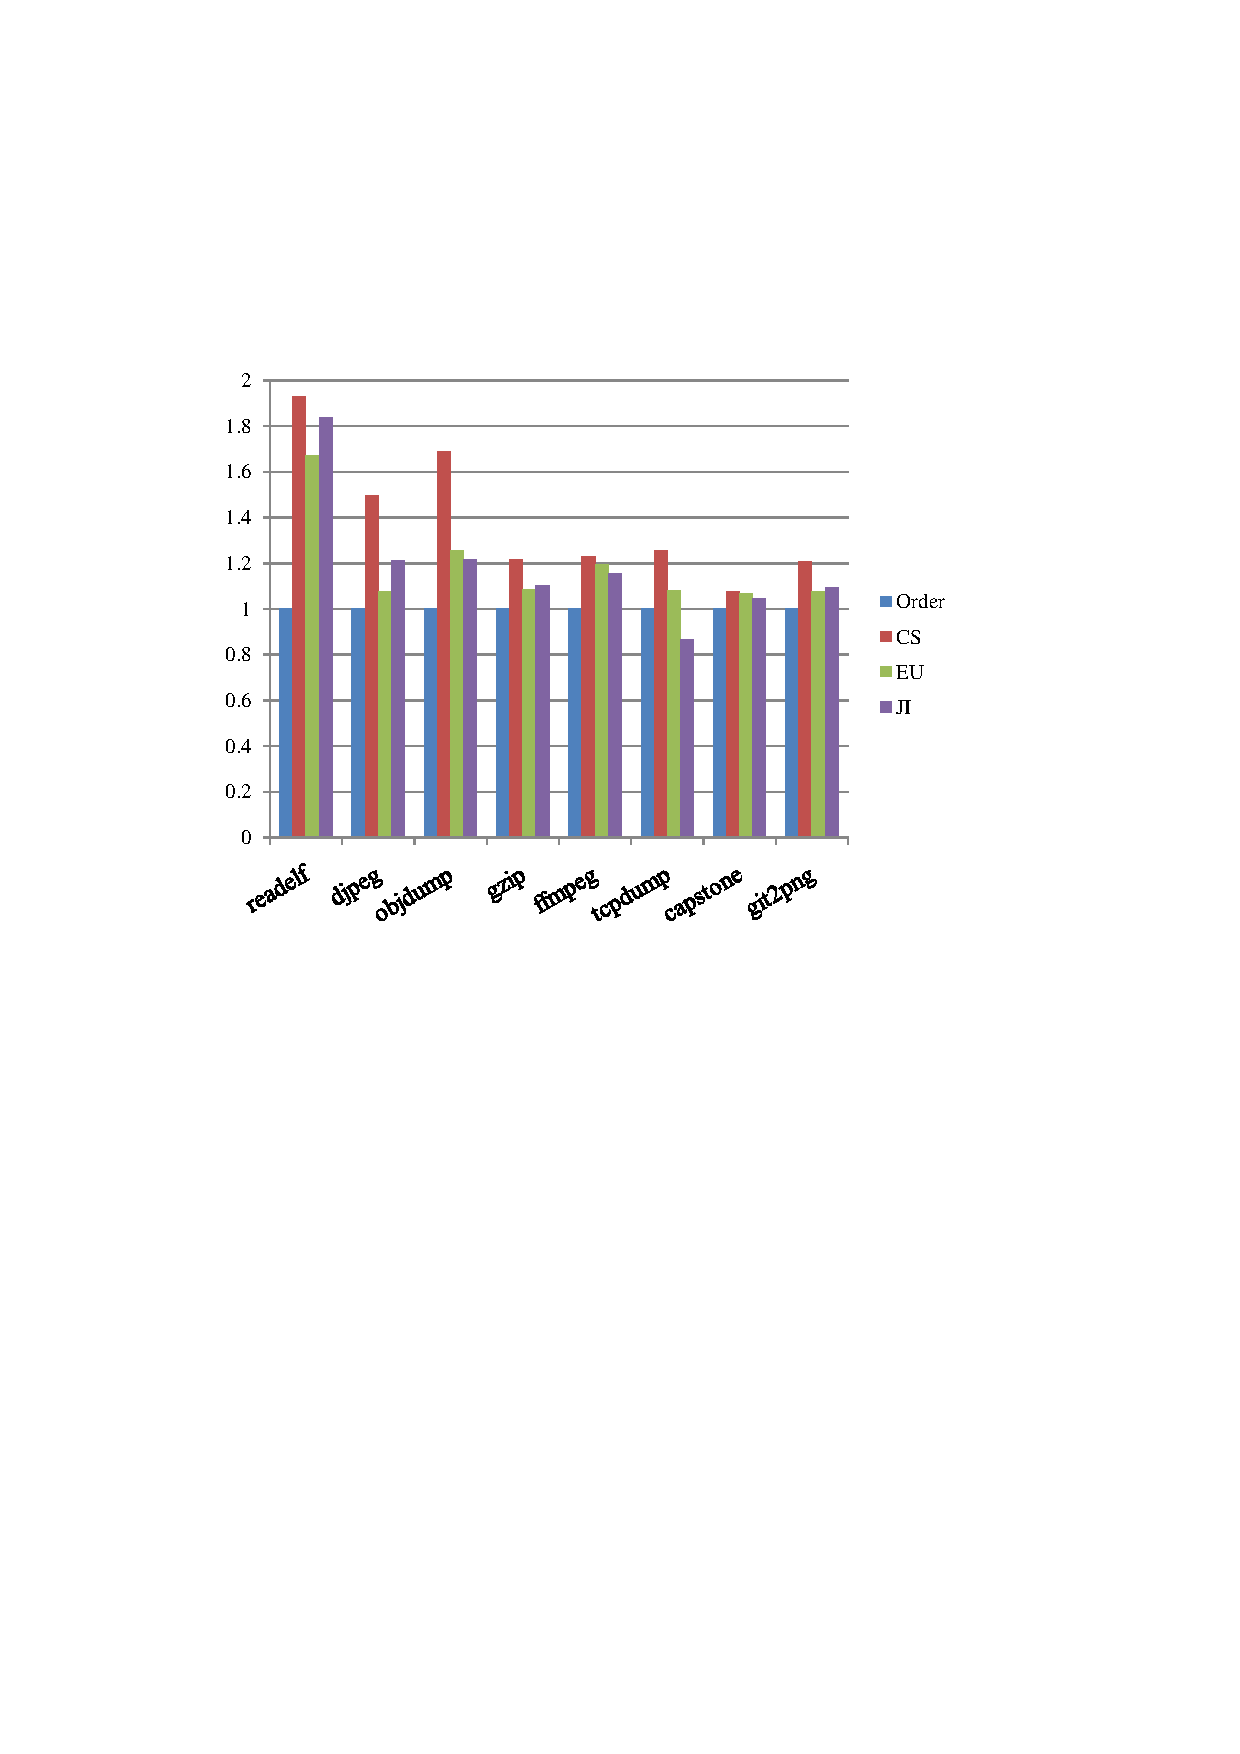
\includegraphics[width=0.45\textwidth, trim={0.2cm 0.4cm 0cm 0cm}, clip]
	{figures/path-discovery.pdf}
	\figfooter{(a)}{Normalized number of unique paths for these 
		four selection strategies to vanilla fuzz testing (i.e., \textit{Order}) }
	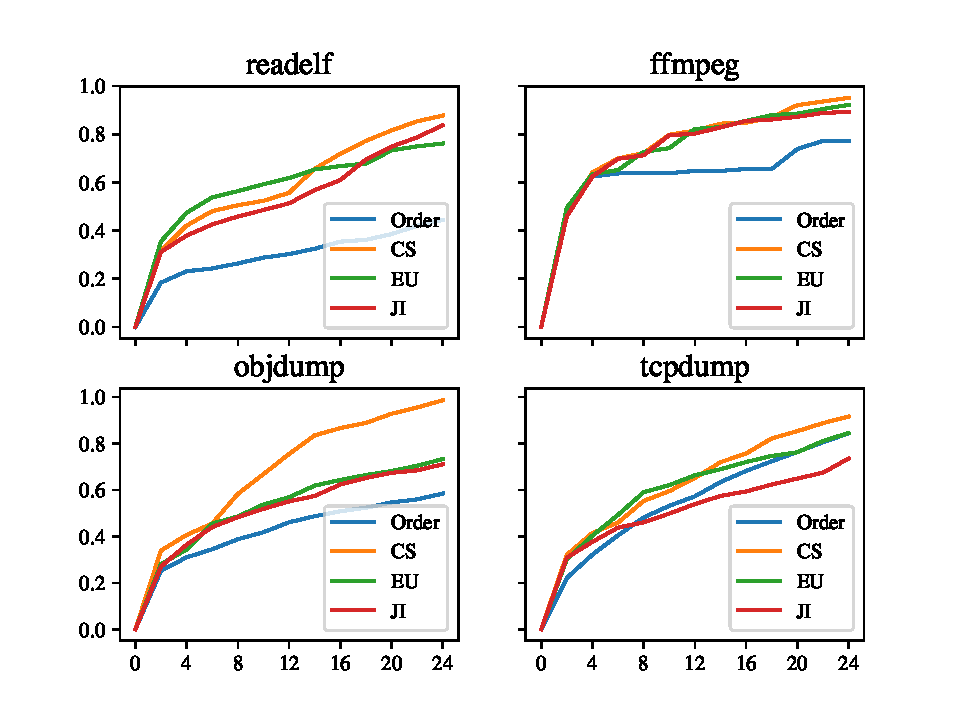
\includegraphics[width=0.45\textwidth, trim={0.15cm 0.1cm 1.5cm 0.8cm}, clip]
	{figures/path-time-detail.pdf} 
	\figfooter{(b)}{Path discovery details along with 24 hours for 
		four sample programs.}\label{fig1}
  \caption{Path discovery results for different seed selection strategies.}
  \label{path-detail}
\end{figure} 

\subsection{Improvement Detail for Each Component (RQ3)} \label{sec:RQ3}
In order to evaluate the contribution of each component on finding 
unique paths, we conducted four experiments (i.e., vanilla AFL fuzz testing, 
symbolic execution assisted hybrid testing (\textit{SEHT}), SEHT with \textit{SPF}, 
SEHT with \textit{SPF\&Searcher}) and compared their results in 24 hours.

In our experiments, since Driller \cite{stephens2016driller} does not support 
real-world binary programs very well now (many library functions and system 
calls are not modeled), we reimplemented the mechanism of Driller within 
S2E to collect the results for SEHT. And based on the results of 
subsection~\ref{sec:RQ2}, our searcher employs cosine similarity 
as the distance metric.

Figure~\ref{path-overall-rsults} summarizes the results of how each 
component contribution to the performance improvement. Compared with 
vanilla fuzz testing, symbolic execution assisted hybrid testing can 
discover 11.88\% more unique paths in average. For example, this 
improvement reaches the highest figure of 42.79\% for \texttt{readelf}. 
However, the performance gain is lower than 20\% for the other 7 programs. 
Specifically, SEHT triggered only 1.32\% more unique paths 
than vanilla fuzz testing for \texttt{gif2png}. This is because the 
symbolic execution engine does not support to handle float number 
operation. After employing \textit{SPF} which handles symbolic pointers 
and symbolic loops, 7.22\% more unique paths touched by SEHT with \textit{SPF}
than SEHT in average. We can see from this figure that 
the performance of SEHT is highly improved by \textit{SPF} 
for \texttt{readelf} and \texttt{objdump} (18.02\% and 22.62\% respectively).
 
This improvement can be continually augmented by cooperating with CS 
searcher (SEHT with \textit{SPF} and CS \textit{Searcher}). For example, the number 
of unique paths discovered by SEHT is increased by 
49.57\% for \texttt{objdump}. In average, the performance of SEHT 
is improved by 24.44\% after introducing \textit{SPF} and CS \textit{Searcher}. From an 
overall viewpoint, \prototype can discover 43.49\% more unique paths 
than vanilla AFL fuzz testing for our benchmark. This improvement is 
because that seeds file with longest distance from already-explored 
spaces have higher likelihood to trigger more fresh branches/paths, 
so solving such seed files earlier by symbolic execution can find more 
fresh seed files than other files. \\

 
Above all, we can obtain that \textit{Searcher} contributes larger 
proportion of contribution to unique path discovery than \textit{SPF}. 
However, this does not mean the contribution of \textit{SPF} is 
negligible. By integrating \textit{SPF} component (i.e., \textit{LCSP} 
and \textit{SLB}), the symbolic execution engine can dive into deeper 
code areas to solve \textit{complex branch conditions} to help fuzzer 
find more fresh paths and discover more hard-to-reach vulnerabilities.

      
\begin{figure}
\begin{center}
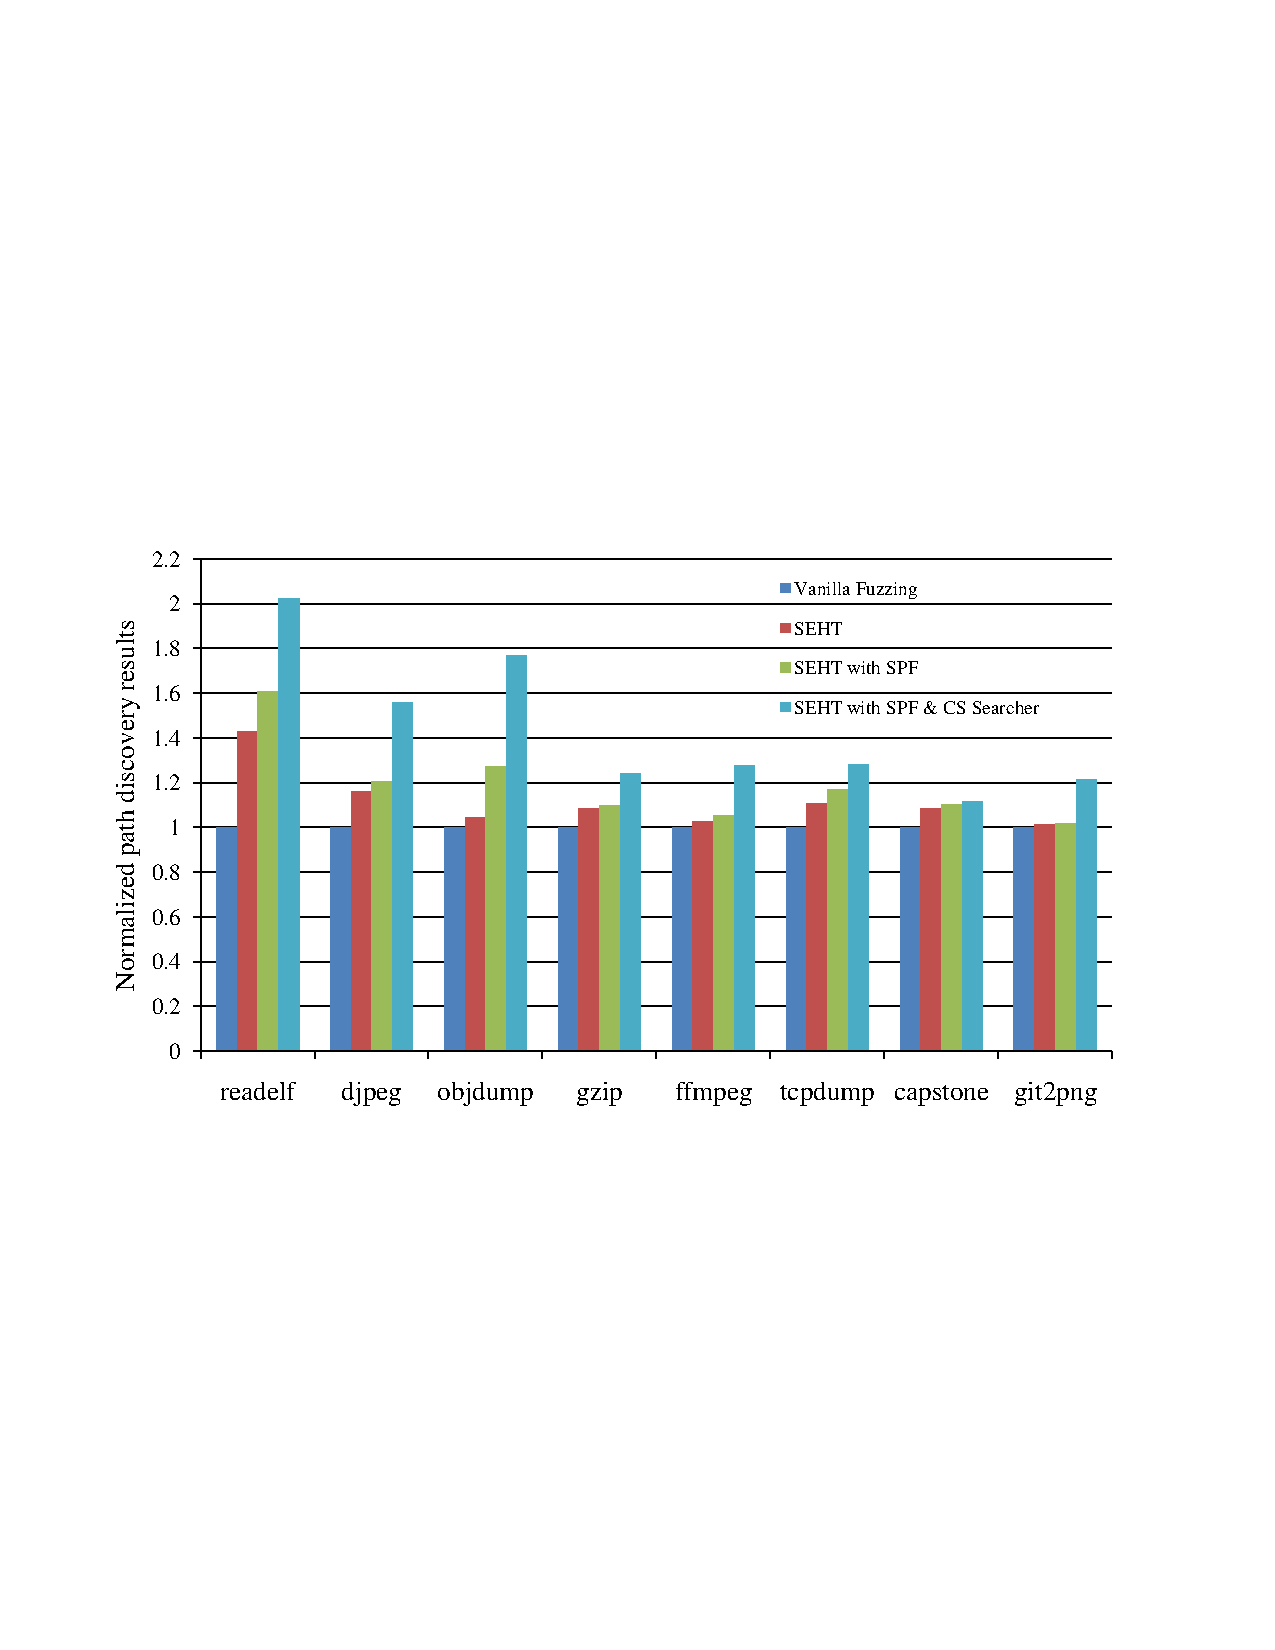
\includegraphics[width=0.5\textwidth]{figures/path-discovery-SPF-CS-all.pdf} 
\caption{Normalized number of unique paths discovered for each component to vanilla fuzz testing.}\label{path-overall-rsults}
\end{center}
\end{figure}

\section{Discussion}
Our method is built on top of fuzz testing and symbolic execution, where we have introduced distance based seed search strategy, symbolic loop bucket, and lazy symbolic pointer. But there are still some drawbacks in our method, so in this section, we will discuss the limitations of our method and take a future look at the vulnerability discovery.

\noindent\textit{\textbf{Distance Measure:}} Our seed search strategy leverages three well-known distance measures, i.e. Euclidean Distance, Cosine Similarity and Jaccard Index. Also, we have evaluated these three measures and compared the results with no search strategy. In the future, we still need to check more definitions of distance, like hamming distance, N-gram distance and so on, to find a better measurement for different execution paths (or different seed inputs). 

\noindent\textit{\textbf{Sanity Check of Symbolic Pointer:}} When given a symbolic pointer, our LSP method will fork a pending state and then continue executing the program until the forking on a branch related to this pending state is failed. Then, we can improve the coverage by scheduling the pending state to generate a new test case. However, a symbolic pointer can point to multiple destinations, our LSP method only focuses on improving the following execution coverage, and because we perform a scale controlled symbolic execution, so we will kill this pending state after the execution is terminated and we will not generate all the possible test cases for this symbolic pointer. This will miss some interesting paths and even bug paths. So, it will be our future work to model the process memory map and then perform assertion checks when encountering with a pending state.

\section{Related Work}
We have presented the major advantages of our method in the previous sections and compared our system with some state-of-the-art vulnerability discovery tools. In this section, we present the techniques that related to our method.

\noindent\textit{\textbf{Similarity Distance in Regression Testing:}}
Similarity based algorithms have been leveraged to regression test case prioritization. Test case prioritization issue is a hot research topic in regression testing research, which tries to optimum mutation schedule based on a specific prioritization criterion. Rothermel et, al. proposed fine-grained prioritization strategy based on the instruction coverage and branch coverage. Then Elbaum et, al. concentrated on function level coverage and they proved that this kind of coarse-grained instrumentation which can reduce the execution overhead but will lose some prioritization performance. Krishna et al. utilized Levenshtein distance as the criterion of prioritization. Rather than using an ordered branch sequence to present the path in [XX], we represented the execution path by using the bitmap in AFL, which is more practical and efficiency.

\noindent\textit{\textbf{Combinational Testing Method:}}
As mentioned before, our method is not the first tool to combine fuzz testing and symbolic execution. Hybrid Fuzz Testing uses symbolic execution to discover frontier nodes that represent unique paths in the program. After collecting as many frontier nodes as possible under a user-specifiable resource constraint, it transits to fuzz the program with random inputs. This tool focuses on binaries but only performs the one-time transition between symbolic execution and fuzz testing. Hybrid Concolic Testing implements multiple transitions between symbolic execution and fuzz testing. But because it is built on top of CUTE, a source code oriented testing tool, so hybrid concolic testing still cannot be deployed on binary testing directly. Driller is an up-to-date hybrid testing tool that leverages fuzz testing and concolic execution in a complementary manner to find deeper bugs. It is more practice when compared with previous hybrid tools. Some other tools try to make full use of symbolic execution to maximize the code coverage, they collect symbolic constraints placed on each input and then negating these constraints to generate a new test case that will take another uncovered path, such as SAGE, Dowser, FuzzWin etc. However, as these tools execute each input in the symbolic mode which determines that they have to face the path explosion problem. 

\section{Conclusion}
In this paper, we proposed a framework built on top of fuzz testing and symbolic execution to improve the performance of path discovery in vulnerability detection for binary executables. In order to achieve this, we introduced three key improvements, i.e. distance based seed search method, symbolic loop bucket and lazy symbolic pointer. The experiments on different benchmarks have shown that by introducing these three key improvements, our framework can find more paths and bugs when compared with other off-the-shelf vulnerability discovery tools. 

\bibliography{biblio.bib}
\bibliographystyle{plain}

\end{document}